\documentclass[letterpaper,final,12pt,reqno]{amsart}

\usepackage[total={6.3in,9.2in},top=1.1in,left=1.1in]{geometry}

\usepackage{times,bm,bbm,empheq,verbatim,fancyvrb,graphicx,amsthm,amssymb}
\usepackage[dvipsnames]{xcolor}
\usepackage{booktabs,multirow,xspace}
\usepackage{pifont}

\usepackage{tabto}
\TabPositions{1.5cm}

\usepackage{tikz}
\usetikzlibrary{decorations.pathreplacing}
\usetikzlibrary{graphs,quotes}

\usepackage[kw]{pseudo}
\pseudoset{%
left-margin=15mm,%
topsep=5mm,%
label=\footnotesize\arabic*,%
idfont=\texttt,%
ctfont=\textsl,%
ct-left=\qquad\qquad(,%
ct-right=),%
}

\usepackage{float}

% hyperref should be the last package we load
\usepackage[pdftex,
colorlinks=true,
plainpages=false, % only if colorlinks=true
linkcolor=blue,   % ...
citecolor=Red,    % ...
urlcolor=black    % ...
]{hyperref}

\renewcommand{\baselinestretch}{1.05}

\allowdisplaybreaks[1]  % allow display breaks in align environments, if they avoid major underfulls

\newtheoremstyle{cstyle}% name
  {5pt}% space above
  {5pt}% space below
  {\itshape}% body font
  {}% indent amount
  {\itshape}% theorem head font
  {.}% punctuation after theorem head
  {.5em}% space after theorem head
  {\thmname{#1}\thmnumber{ #2}\thmnote{ (#3)}}% theorem head spec
\theoremstyle{cstyle}

\newtheorem{theorem}{Theorem}
\newtheorem{lemma}[theorem]{Lemma}
\newtheorem{corollary}[theorem]{Corollary}
\newtheorem{assumptions}[theorem]{Assumptions}

\newtheoremstyle{cstyle*}% name
  {5pt}% space above
  {5pt}% space below
  {\itshape}% body font
  {}% indent amount
  {\itshape}% theorem head font
  {.}% punctuation after theorem head
  {.5em}% space after theorem head
  {\thmname{#1}}% theorem head spec
\theoremstyle{cstyle*}
\newtheorem{assumptions*}{Assumptions}

\newtheoremstyle{dstyle}% name
  {5pt}% space above
  {5pt}% space below
  {}%{\itshape}% body font
  {}% indent amount
  {\itshape}% theorem head font
  {.}% punctuation after theorem head
  {.5em}% space after theorem head
  {\thmname{#1}\thmnumber{ #2}\thmnote{ (#3)}}% theorem head spec
\theoremstyle{dstyle}

\newtheorem{definition}[theorem]{Definition}
\newtheorem{example}[theorem]{Example}

% numbering
\numberwithin{equation}{section}
\numberwithin{figure}{section}
\numberwithin{table}{section}
\numberwithin{theorem}{section}

\newcommand{\eps}{\epsilon}
\newcommand{\RR}{\mathbb{R}}

\newcommand{\grad}{\nabla}
\newcommand{\Div}{\nabla\cdot}
\newcommand{\trace}{\operatorname{tr}}

\newcommand{\hbn}{\hat{\mathbf{n}}}

\newcommand{\bb}{\mathbf{b}}
\newcommand{\be}{\mathbf{e}}
\newcommand{\bbf}{\mathbf{f}}
\newcommand{\bg}{\mathbf{g}}
\newcommand{\bn}{\mathbf{n}}
\newcommand{\br}{\mathbf{r}}
\newcommand{\bu}{\mathbf{u}}
\newcommand{\bv}{\mathbf{v}}
\newcommand{\bw}{\mathbf{w}}
\newcommand{\bx}{\mathbf{x}}
\newcommand{\by}{\mathbf{y}}
\newcommand{\bz}{\mathbf{z}}

\newcommand{\bF}{\mathbf{F}}
\newcommand{\bV}{\mathbf{V}}
\newcommand{\bX}{\mathbf{X}}

\newcommand{\bxi}{\bm{\xi}}
\newcommand{\bzero}{\bm{0}}

\newcommand{\cK}{\mathcal{K}}
\newcommand{\cV}{\mathcal{V}}

\newcommand{\rhoi}{\rho_{\text{i}}}

\newcommand{\ip}[2]{\langle#1,#2\rangle}

\newcommand{\maxR}{R^{\bm{\oplus}}}
\newcommand{\minR}{R^{\bm{\ominus}}}
\newcommand{\iR}{R^{\bullet}}

\newcommand{\nn}{{\text{n}}}
\newcommand{\pp}{{\text{p}}}
\newcommand{\qq}{{\text{q}}}
\newcommand{\rr}{{\text{r}}}

\newcommand{\supp}{\operatorname{supp}}
\newcommand{\Span}{\operatorname{span}}

\newcommand{\fascd}{\pr{fascd}\xspace}

\newcommand{\rNC}{r_{\text{NC}}}
\newcommand{\rSS}{r_{\text{SS}}}
\newcommand{\rXX}{r_{\text{XX}}}

\newcommand{\XX}{\ding{55}}

\newcommand{\dx}{\, \mathrm{d}x}
\DeclareMathOperator*{\argmin}{arg\,min}

\newfloat{pseudofloat}{t}{xyz}[section]
\floatname{pseudofloat}{Algorithm}

\usepackage{todonotes}
\newcommand{\pef}[1]{\todo[inline, color=red!20]{PF: #1}}
\newcommand{\elb}[1]{\todo[inline, color=blue!20]{EB: #1}}


\begin{document}
\title[FAS for nonlinear variational inequalities]{A full approximation scheme multilevel method \\ for nonlinear variational inequalities}

\author{Ed Bueler}

\author{Patrick E.~Farrell}

\date{\today}

\begin{abstract}
We present the \emph{full approximation scheme constraint decomposition} (FASCD) multilevel method for solving variational inequalities (VIs).  FASCD is a common extension both of the full approximation scheme (FAS) multigrid technique for nonlinear partial differential equations, due to A.~Brandt, and the constraint decomposition (CD) method introduced by X.-C.~Tai for VIs arising in optimization.  We extend the CD idea by exploiting the telescoping nature of certain function space subset decompositions arising from multilevel mesh hierarchies.  We demonstrate that FASCD V-cycles exhibit excellent mesh-independent convergence rates.  Furthermore, when a reduced-space active set method is applied as a smoother, with work proportional to the number of unknowns on a given mesh level, FASCD F-cycles (full multigrid) are optimal solvers.  The example problems include differential operators which are symmetric linear, nonsymmetric linear, and nonlinear, in unilateral and bilateral VI problems.  Our examples demonstrate very good convergence even on problems where other multilevel VI solvers struggle.
\end{abstract}

\maketitle

\thispagestyle{empty}


\section{Introduction} \label{sec:intro}

The constraint decomposition (CD) methods of Tai \cite{Tai2003} are designed to solve coercive variational inequality (VI) problems arising as the Karush--Kuhn--Tucker optimality conditions for the minimization of a convex functional over a convex set.  These methods were shown to converge for multilevel and domain decompositions in a finite element (FE) context.  In the multilevel case, this CD method has almost grid-independent error bounds, and near-optimal complexity, for elliptic, linear obstacle problems \cite[Subsection 5.4]{Tai2003}, \cite[Theorem 4.6 and Algorithm 4.7]{GraeserKornhuber2009}.

Here we extend Tai's multilevel CD method by replacing the coarser-level corrections with a full approximation scheme (FAS; \cite{Brandt1977,Bruneetal2015}) approach.  Specifically, our \emph{full approximation scheme constraint decomposition} (FASCD) method extends the \cite{GraeserKornhuber2009,Tai2003} algorithms in the following directions:
\renewcommand{\labelenumi}{\emph{(\roman{enumi})}}
\begin{enumerate}
\item The FAS coarse corrections are adapted for general VI problems. The needed computations require neither an objective function nor linearity of the residual operator.
\item Box constraints (i.e.~both upper and lower obstacles) are allowed.
\item As with the original CD method \cite{Tai2003}, but unlike some implementations \cite[for example]{GraeserKornhuber2009}, and semismooth methods generally \cite{BensonMunson2006,Ulbrich2011}, the method can be applied even if the residual operator is defined only on those functions which satisfy the constraints.
\pef{I confess I find this explicit calling out of other algorithms a bit uncomfortable/too much. I wonder if the following is better?}
\item The method is strictly admissible, and so can be applied even if the residual operator is defined only on those functions which satisfy the constraints.
\item V-cycles (Algorithm \ref{alg:fascd}) and F-cycles (full multigrid; Algorithm \ref{alg:fascd-fcycle}) are implemented.
\item We identify a ``telescoping'' subset property which can be exploited on the up-smoothing side of a V-cycle for greater performance.
\item When used in conjunction with a reduced-space active set method as a smoother, we demonstrate that F-cycle FASCD is an optimal solver for the different VI examples in Section \ref{sec:results}.  The work of the smoother is proportional to the number of unknowns on a given level because the number of Newton and Krylov iterations is fixed.
\end{enumerate}

Prior multilevel algorithms for VIs have various substantial limitations compared to the FASCD framework.  The projected full approximation scheme (PFAS) algorithm of Brandt \& Cryer \cite{BrandtCryer1983} is apparently limited to linear complementarity problems and projected (truncated) Gauss--Seidel smoothers.  While FASCD reduces to general, nonlinear FAS for PDEs when the inequality constraints are removed (Appendix \ref{app:reductions}), PFAS reduces to linear multigrid.  The multilevel CD iteration of Tai \cite{Tai2003} is formulated in terms of an objective function, so it only applies to optimization-type problems, and furthermore each of its coarser-level problems refers to the finest-level discretization.  The latter property is improved by reformulation using defect constraints and monotone injection operators (see \cite[Algorithm 4.7]{GraeserKornhuber2009}, or Section \ref{sec:cdmultilevel} herein).  The monotone multigrid methods of Kornhuber and co-authors \cite{GraeserKornhuber2009,Kornhuber1994} appear to be formulated only with Gauss--Seidel type smoothers, and applied only to optimization-type VI problems \cite[for example]{JouvetGraeser2013}.  Furthermore, monotone multigrid methods are more difficult to implement in FE libraries because modifications of the FE basis functions are needed to approximate the coarser-level coincidence sets.  \pef{My current understanding is that this refers to \emph{truncated} monotone multigrid; monotone multigrid just means using monotone injection operators appropriately. Let me double-check. And my understanding is that the `modification' of the basis functions is just zeroing the basis functions for vertices in the active set, so you don't have to modify the basis functions, just zero some rows/columns of the matrix.} No such invasive basis modifications are used either in Tai's CD, nor in our Firedrake library \cite{Rathgeberetal2016} implementation of FASCD.  However, our implementation exceeds monotone multigrid performance, including on a problem used to demonstrate the benefits of that method (Example \ref{ex:results:classical}; compare \cite[problem 7.1.1]{GraeserKornhuber2009}).

Regarding its limitations, FASCD solves only bound-constrained VI problems.  The method differs from the original FAS method only if the constraint set is proper (Appendix \ref{app:reductions}).

In our experiments, FASCD V-cycles exhibit essentially the same mesh-independent convergence rates for VI problems that FAS multigrid V-cycles exhibit for corresponding unconstrained PDE problems.  The F-cycle results in Section \ref{sec:results} show nearly-textbook multigrid efficiency, namely solutions within discretization error in work comparable to few smoother sweeps on the finest-level mesh \cite{BrandtLivne2011}.  Specifically, we see this performance for classical (unilateral, Laplacian) obstacle problems, $p$-Laplacian obstacle problems, and box-constrained advection-diffusion equations.  Furthermore, these results appear to be insensitive to the length or structure of the free boundary, i.e.~the geometric complexity of the coincidence set.

All iterates in FASCD are admissible, and thus the nonlinear operator in the VI needs only be defined for admissible states.  For example, we solve an ice sheet geometry problem (Examples \ref{ex:sia} and \ref{ex:results:sia}) in which the ice flow formulas are only meaningful for surface elevation iterates that do not penetrate the bedrock.  Non-admissible methods, including semi-smooth methods \cite{BensonMunson2006}, would require unnatural modifications of the operator formula.  FASCD solves this low-regularity ice sheet problem, wherein the solution has unbounded gradient at the free boundary, by a small, mesh-independent number of F-cycle iterations (Example \ref{ex:results:sia}).

\elb{beam 2d example?}

The paper is organized as follows.  In Section \ref{sec:vi} we recall the theory of coercive and monotone variational inequalities, and describe several motivating examples.  Section \ref{sec:cd} reviews the basics of CDs and their associated iterations.  Section \ref{sec:femultilevel} sets up multilevel FE hierarchies, and then Section \ref{sec:cdmultilevel} extends the CD method via defect constraints generated by monotone injection operators \cite{GraeserKornhuber2009}.  Here we propose an apparently new understanding of telescoping sets for up-smoothing, based on an ``incomplete'' CD and an associated iteration.  Section \ref{sec:vcycle} then states the FASCD V-cycle, with Section \ref{sec:implementation} addressing convergence criteria, F-cycles, and our smoother choice.  Section \ref{sec:results} gives numerical results from a parallel Firedrake \cite{Rathgeberetal2016} implementation (see Code Availability), for each example problem introduced in Section \ref{sec:vi}.  The work concludes with a discussion and outlook in Section \ref{sec:discussion}.


\section{Variational inequalities} \label{sec:vi}

Let $\cV$ be a real and reflexive Banach space with norm $\|\cdot\|$ and topological dual space $\cV'$.  Denote the dual pairing of $\phi \in \cV'$ and $v\in\cV$ by $\ip{\phi}{v} = \phi(v)$, and define the (Banach space) norm on $\cV'$ by $\|\phi\|' = \sup_{\|v\|=1} |\ip{\phi}{v}|$.  Let $\cK \subset \cV$ be a nonempty, closed, and convex subset, the \emph{constraint set}; elements of $\cK$ are said to be \emph{admissible}.  For a continuous, but generally nonlinear, operator $f:\cK \to \cV'$ and a linear \emph{source functional} $\ell\in \cV'$ we consider the following \emph{variational inequality} (VI) problem: find $u^\star\in \cK$ such that
\begin{equation}
\ip{f(u^\star)}{v-u^\star} \ge \ip{\ell}{v-u^\star} \quad \text{for all } v\in \cK. \label{eq:vi}
\end{equation}
Because $f$ is (generally) nonlinear, the source term $\ell$ is not strictly needed in stating this class of problems.  In fact, by redefining $f$ we may take $\ell=0$.  However, introducing $\ell$ clarifies the algorithm in Section \ref{sec:vcycle}.

VI \eqref{eq:vi} generalizes nonlinear systems of equations $f(u^\star)=\ell$ to problems where $u^\star$ is also constrained to be in $\cK$.  Informally, pretending the dual pairing is an inner product, \eqref{eq:vi} says that the angle between $f(u^\star)-\ell$ and any arbitrary vector $v-u^\star$ pointing from $u^\star$ into $\cK$ is at most $90^\circ$; while $f(u^\star)-\ell$ may not be zero, it must point directly into $\cK$.  On the other hand, if $u^\star$ is in the interior of the constraint set then \eqref{eq:vi} implies $f(u^\star)=\ell$.
Variational inequalities may generally permit multiple solutions~\cite{Farrell2019}.

The following definitions are standard \cite{KinderlehrerStampacchia1980}.

\begin{definition}  A map $f:\cK \to \cV'$ is \emph{monotone} if
\begin{equation}
\ip{f(u)-f(v)}{u-v} \ge 0 \qquad \text{for all } u,v \in \cK, \label{eq:monotone}
\end{equation}
\emph{strictly monotone} if equality in \eqref{eq:monotone} implies $u=v$, and \emph{coercive} if there exists $w \in \cK$ so that
\begin{equation}
\frac{\ip{f(u)-f(w)}{u-w}}{\|u-w\|} \to +\infty \qquad \text{as } \|u\|\to +\infty. \label{eq:coercive}
\end{equation}
\end{definition}

It is well-known that if $f:\cK \to \cV'$ is continuous, monotone, and coercive then VI \eqref{eq:vi} has a solution \cite[Corollary III.1.8]{KinderlehrerStampacchia1980}, and that the solution is unique when $f$ is strictly monotone.  As is standard in the calculus of variations \cite{Evans2010}, coercivity permits a compactness argument for unbounded sets $\cK$.  (Recall that the closed and bounded subsets of a reflexive Banach space are weakly compact.)  The condition of continuity can be weakened, e.g.~to only apply on finite-dimensional subspaces \cite{KinderlehrerStampacchia1980}, but this is unnecessary in our examples.

Some of the VIs solved in this paper satisfy a stronger inequality than \eqref{eq:coercive}.

\begin{definition}  Let $p>1$.  The map $f:\cK \to \cV'$ is \emph{$p$-coercive} if there exists $\kappa>0$ such that
\begin{equation}
\ip{f(u)-f(v)}{u-v} \ge \kappa \|u-v\|^p \qquad \text{for all } u,v \in \cK. \label{eq:pcoercive}
\end{equation}
\end{definition}

It is easy to see that if $f$ is $p$-coercive then it is monotone, strictly monotone, and coercive, so the following well-posedness theorem holds.

\begin{theorem}  \label{thm:viwellposed}  If $f:\cK \to \cV'$ is continuous and $p$-coercive then there exists a unique $u^\star\in \cK$ solving VI \eqref{eq:vi}.
\end{theorem}

Let $\Omega \subset \RR^d$ denote a bounded, open set with smooth or piecewise-smooth (e.g.~polygonal) boundary.  Sobolev spaces \cite{Evans2010} will be denoted by $W^{k,p}(\Omega)$, for integer $k$ and $1\le p \le \infty$, with $W^{1,p}_0(\Omega)$ denoting the subspace having zero boundary values.

The following example includes the classical and $p$-Laplacian obstacle problems \cite{ChoeLewis1991}.

\begin{example}  \label{ex:plaplacian}  Let $p>1$.  For $u,v \in \cV = W^{1,p}_0(\Omega)$, define $f:\cV \to \cV'$ by
\begin{equation}
\ip{f(u)}{v} = \int_\Omega |\grad u|^{p-2} \grad u \cdot \grad v\dx, \label{eq:plaplacian}
\end{equation}
a continuous map \cite[Theorem A.0.6]{Peral1997}.  For $p\ge 2$, if $x,y\in\RR^d$ then $(|x|^{p-2} x - |y|^{p-2} y)\cdot (x-y) \ge 2^{2-p} |x-y|^p$ \cite[Appendix A]{Bueler2021conservation}, hence it follows from the Poincar\'e inequality that
    $$\ip{f(u) - f(v)}{u-v} \ge 2^{2-p} a_0 \|\grad u - \grad v\|_p^p \ge 2^{2-p} a_0 C \|u-v\|^p$$
for some $C>0$, and thus $f$ is $p$-coercive.  The map \eqref{eq:plaplacian} is also coercive if $1<p<2$, but the proof is somewhat different \cite[Theorem 4.4, for example]{Bueler2021conservation}.  \end{example}

For monotone operators $f$, VI \eqref{eq:vi} generalizes the problem of minimizing a convex function over $\cK$.  In fact, suppose $F:\cK \to \RR$ is lower semi-continuous and (G\^ateau) differentiable with continuous derivative $F':\cK \to \cV'$.  Then $F$ is convex if and only if $F'$ is monotone \cite[Proposition I.5.5]{EkelandTemam1976}.  Furthermore, Proposition II.2.1 in \cite{EkelandTemam1976} shows that if $F$ is convex then \eqref{eq:vi} holds for $f=F'$ if and only if
\begin{equation}
u^\star = \argmin_{v\in\cK} F(v) - \ip{\ell}{v}. \label{eq:minimization}
\end{equation}
The CD methods of Tai \cite{Tai2003} address problem \eqref{eq:minimization}; the analysis in \cite{Tai2003} supposes that an objective $F$ exists with $F'$ 2-coercive.  For Example \ref{ex:plaplacian} we may define
\begin{equation}
F(v) = \frac{1}{p} \int_\Omega |\grad v|^p\dx. \label{eq:plaplacianobjective}
\end{equation}
Then $F$ is a convex functional and $F'(v) = f(v)$ for $f$ given in \eqref{eq:plaplacian}.  For any closed and convex $\cK\subset \cV$, VI problem \eqref{eq:vi} is then equivalent to optimization problem \eqref{eq:minimization}.

Next we give two examples which are \emph{not} of optimization type \eqref{eq:minimization}, the first being an advection-diffusion problem, which needs the following Lemma.

\begin{lemma}  \label{lem:advectionskew}  \cite{Elmanetal2014}\,  Suppose $\bX :\Omega \to \RR^d$ is a bounded and boundedly-differentiable vector field on $\Omega$ with zero divergence ($\Div \bX=0$).  For $u,v \in W^{1,2}(\Omega)$ let $b(u,v) = \int_\Omega (\bX \cdot \grad u) v\dx$.  Then $b(u,u) = \frac{1}{2} \int_{\partial \Omega} u^2 \bX\cdot \bn\dx$ where $\bn$ is the outward normal on $\partial \Omega$.
\end{lemma}

\begin{proof}
Integration by parts gives $b(u,v) = - b(v,u) + \int_{\partial \Omega} uv \bX\cdot \bn\dx$.
\end{proof}

\begin{example}  \label{ex:advectiondiffusion}  Suppose $\partial\Omega$ is partitioned into Dirichlet and Neumann portions, i.e.~$\partial\Omega = \partial_D\Omega \cup \partial_N\Omega$, with $\partial_D\Omega$ of positive Hausdorff measure.  Let $\cV \subset W^{1,2}(\Omega)$ be the space of functions which are zero along $\partial_D\Omega$.  Consider a divergence-free velocity field $\bX$ on $\Omega$ satisfying the conditions of Lemma \ref{lem:advectionskew}, and assume that the flow is outward on the Neumann boundary: $\bX \cdot \bn \ge 0$ on $\partial_N\Omega$.  For $u,v \in \cV$, $\eps>0$, and $\phi \in \cV'$, define
\begin{equation}
\ip{f(u)}{v} = \eps \left(\grad u, \grad v\right)_{L^2(\Omega)} + b(u,v) - \ip{\phi}{v}. \label{eq:advectiondiffusion}
\end{equation}
With this operator, consider VI \eqref{eq:vi} with $\ell = 0$ for any closed and convex $\cK \subset \cV$. The interior condition, i.e.~PDE strong form, is the following linear advection-diffusion equation
\begin{equation}
-\eps \grad^2 u + \bX\cdot \grad u = \phi.
\label{eq:advectiondiffusionstrong}
\end{equation}
On the other hand, it is easy to see that $|\ip{f(u)}{v}| \le \left((\eps + \|\bX\|_\infty) \|u\| + \|\phi\|'\right) \|v\|$, so that $f:\cK \to \cV'$ is continuous.  Lemma \ref{lem:advectionskew} says that the bilinear form $b(u,v)$ is skew-symmetric up to a nonnegative term.  By the outward flow assumption and the Poincar\'e inequality,
\begin{align*}
\ip{f(u)-f(v)}{u-v} &= \eps \int_\Omega |\grad u - \grad v|^2\dx + b(u-v,u-v) \\
                    &= \eps \int_\Omega |\grad u - \grad v|^2\dx + \frac{1}{2} \int_{\partial_N\Omega} (u-v)^2 \bX\cdot\bn \ge \eps C \|u-v\|^2.
\end{align*}
Thus $f$ is 2-coercive, and so the associated VI problem is well-posed.
\end{example}

If $\bX \ne 0$ then $f\ne F'$ for any objective $F$, because $\ip{f(u)}{v}$ does not possess the symmetry of the gradient of a scalar: for $u,v$ which are zero on $\partial \Omega$, note that $\ip{f(u)}{v} - \ip{f(v)}{u} = -2 b(u,v)$.  References \cite{Bueler2021conservation,ChangNakshatrala2017} consider inequality-constrained advection-diffusion VI problems like this, specifically over the set $\cK = \{v\ge 0\}$.

The next VI example is a model for steady ice sheet geometry in a given climate. It is nonlinear and not of optimization type. Related VI problems arise for any fluid layer which is subject to boundary processes that can remove fluid mass \cite{Bueler2021conservation}.

\begin{example}  \label{ex:sia}  Let $\Omega \subset \RR^2$ be a fixed region of land, and suppose $b \in C^1(\Omega)$ is a given bedrock elevation.  Let $a \in L^2(\Omega)$ denote a given ``surface mass balance'' function, the annually-averaged rate of ice accumulation (as snow) minus melt and runoff.  Then the surface elevation $s\in C(\Omega)$ of a steady-state, isothermal, and non-sliding ice sheet (glacier) approximately satisfies the following \emph{shallow ice approximation} (SIA) \cite{GreveBlatter2009} VI problem: find $s \in \mathcal{K} = \{s\ge b\}$ such that
\begin{equation}
\int_\Omega \Gamma (s-b)^{n+2} |\grad s|^{n-1} \grad s \cdot \grad (v-s) \dx \ge \int_\Omega a (v-s)\dx \quad \text{ for all } v \in \mathcal{K}, \label{eq:siavi}
\end{equation}
where $n>1$ and $\Gamma>0$ are constants determined by the physical properties of ice; $n=3$ is a typical value.  The doubly-nonlinear and doubly-degenerate operator in this case is
\begin{equation}
\ip{f(s)}{v} = \int_\Omega \Gamma (s-b)^{n+2} |\grad s|^{n-1} \grad s \cdot \grad v\dx. \label{eq:sia}
\end{equation}
If the bed is flat ($b=0$) then a power transformation converts the problem into $p$-Laplacian form \eqref{eq:plaplacian} with $p=n+1$.  For general beds $b$ less is understood about this operator, but existence holds for \eqref{eq:siavi} \cite{JouvetBueler2012} and a power of the solution lives in a Sobolev space: $(s-b)^{2p/(p-1)} \in W^{1,p}(\Omega)$.  This theory, and also observations of ice sheets, shows that $|\grad s|$ is generally unbounded as one approaches the free boundary from the icy ($s>b$) side.
\end{example}

Numerical results are shown in Section \ref{sec:results} for applications of FASCD Algorithms \ref{alg:fascd} and \ref{alg:fascd-fcycle} to these Examples.


\section{Constraint decomposition (CD)} \label{sec:cd}

Suppose that there are $m<\infty$ closed subspaces $\cV_i \subset \cV$, so that the sum
\begin{equation}
\cV = \sum_{i=0}^{m-1} \cV_i \label{eq:subspacedecomp}
\end{equation}
holds in the sense that if $w \in \cV$ then there exist $w_i \in \cV_i$ so that $w = \sum_i w_i$.  We say \eqref{eq:subspacedecomp} is a \emph{space decomposition} of $\cV$ \cite{Xu1992}.  For a closed, convex subset $\cK \subset \cV$, suppose further that $\cK_i \subset \cV_i$ are nonempty, closed, and convex subsets such that
\begin{equation}
\cK = \sum_{i=0}^{m-1} \cK_i. \label{eq:constraintdecomp}
\end{equation}
The sum in \eqref{eq:constraintdecomp} must hold in two senses \cite{TaiTseng2002}: \emph{(i)}~if $w \in \cK$ then there exist $w_i \in \cK_i$ so that $w = \sum_i w_i$, and \emph{(ii)}~if $z_i \in \cK_i$ for each $i$ then $\sum_i z_i \in \cK$.  Note that neither decomposition \eqref{eq:subspacedecomp} or \eqref{eq:constraintdecomp} is required to be unique, and also notice that sense \emph{(ii)} is automatic for \eqref{eq:subspacedecomp} because the $\cV_i$ are subspaces.  Finally, suppose there are bounded, generally nonlinear, \emph{decomposition operators}\footnote{Denoted ``$R_i$'' in \cite{Tai2003}.  Here we avoid a notational conflict with multilevel transfer operators (Section \ref{sec:femultilevel}).} $\Pi_i : \cK \to \cK_i$ such that if $v \in \cK$ then
\begin{equation}
v = \sum_{i=0}^{m-1} \Pi_i v.  \label{eq:constraintrestrictionsum}
\end{equation}
Clearly \eqref{eq:constraintrestrictionsum} implies sense \emph{(i)} for \eqref{eq:constraintdecomp}.  A \emph{constraint decomposition} (CD) of $\cK$ is a choice of $\cV_i,\cK_i,\Pi_i$ satisfying \eqref{eq:subspacedecomp}--\eqref{eq:constraintrestrictionsum} \cite{Tai2003}.  Figure \ref{fig:cartoon} suggests how a low-dimensional example might look; note $\cK_i \not\subset \cK$ in this and most other cases.

\begin{figure}[ht]
\includegraphics[width=0.6\textwidth]{genfigs/cartoon.pdf}
\caption{A constraint decomposition (CD) for a unilateral obstacle problem on a two-point space $\Omega=\{x_1,x_2\}$, with $\mathcal{V}=\left\{v \,:\, \Omega \to \RR\right\}$ and $\mathcal{K}=\{v\ge \psi\}$.}
\label{fig:cartoon}
\end{figure}

In Sections \ref{sec:femultilevel}--\ref{sec:vcycle} we will introduce multilevel FE CD discretizations and algorithms for finite-dimensional VI problems.  However, the CD concept applies at the level of the continuum problem, as illustrated in the following two examples.  The first example is an overlapping domain decomposition of a Sobolev space.  Again note that $\cK_i \not\subset \cK$; informally speaking, the important inclusion is $\cK_i \subset \cV_i$.

\begin{example}  \label{ex:domaindecomposition}  For a bounded domain $\Omega \subset \RR^d$, let $\cV = W_0^{k,p}(\Omega)$ for $k\ge 0$ and $p\ge 1$.  Let $\psi$ be a measurable, real-valued obstacle, defined on $\Omega$, which satisfies $\psi|_{\partial \Omega} \le 0$, and let $\cK = \{v \ge \psi\} \subset \cV$.  Suppose that $\{\phi_i\}_{i=0}^{m-1}$ is a smooth partition of unity on $\Omega$, satisfying $0 \le \phi_i\le 1$ and $\sum_i \phi_i = 1$, and let $\Omega_i$ be the open support of $\phi_i$.  Let $\cV_i = \{w \in \cV:w|_{\Omega \setminus \Omega_i} =0 \}$, $\cK_i = \{v \in \cV_i: v \ge \phi_i \psi\}$, and $\Pi_i(v) = \phi_i v$.  Then \eqref{eq:subspacedecomp}--\eqref{eq:constraintrestrictionsum} hold, giving a CD.
\end{example}

Our second example is a disjoint frequency decomposition of a Hilbert space.  A multilevel CD over a finite-dimensional FE discretization (Sections \ref{sec:femultilevel}--\ref{sec:cdmultilevel}) should approximate this CD.

\begin{example}  \label{ex:frequencydecomposition}  Suppose $\Omega = (0,a)^d \subset \RR^d$ is a cube, and let $\cV = W_{\text{per}}^{2,k}(\Omega)$ be the periodic functions with square-integrable $k$th derivatives, for $k \ge 0$.  Suppose $\psi \in W_{\text{per}}^{2,k}(\Omega)$ and let $\cK = \{v \ge \psi\} \subset \cV$.  Without using any detailed notation for Fourier representation, but noting that the frequencies are discrete because $\Omega$ is compact, suppose $\{\cV_i\}$ are $m<\infty$ subspaces of $\cV$ defined by an (nonoverlapping) partition of $W_{\text{per}}^{2,k}(\Omega)$ by frequency, thus satisfying \eqref{eq:subspacedecomp} as an orthogonal decomposition.  Suppose $P_i:\cV \to \cV_i$ are the corresponding orthogonal projections, satisfying $I = \sum_i P_i$.  Let $\cK_i = \{v \ge P_i \psi\} \subset \cV_i$ and $\Pi_i = P_i$.  Then \eqref{eq:constraintdecomp} and \eqref{eq:constraintrestrictionsum} also hold.
\end{example}

Associated to any CD are certain iterative methods \cite{Tai2003,Xu1992}.  Let $0\le \alpha \le 1$ be the \emph{damping parameter}.\footnote{FASCD Algorithms \ref{alg:fascd} and \ref{alg:fascd-fcycle} are presented without damping, and indeed it seems to be unnecessary.  However, the convergence of the general CD iterations appears to depend upon it.}  The following algorithms, which replace $u \in \cK$ with a new iterate $w\in\cK$ which should be closer to $u^\star \in \cK$ solving \eqref{eq:vi}, solve smaller VI problems over each subset $\cK_i$.

The additive/parallel \pr{cd-add} algorithm generalizes the classical Jacobi iteration.  In its VI problem the expression ``$u-\Pi_iu+\hat w_i$'' removes the part of $u$ which lies in $\mathcal{K}_i$, and then adds-back the subset solution $\hat w_i \in \mathcal{K}_i$.

\begin{pseudo*}
\pr{cd-add}(u)\text{:} \\+
    for all $i \in \{0,\dots,m-1\}$: \\+
        \rm{find} $\hat w_i\in \cK_i$ \rm{such that} \\+
            $\ip{f(u - \Pi_i u + \hat w_i)}{v_i-\hat w_i} \ge \ip{\ell}{v_i-\hat w_i} \textnormal{ for all } v_i \in \cK_i$ \\--
    $\hat w = \sum_i \hat w_i\in\cK$ \\
    return $w=(1-\alpha) u + \alpha \hat w$
\end{pseudo*}

The multiplicative/successive \pr{cd-mult} algorithm generalizes the Gauss--Seidel iteration.  Each subset solution corrects the global iterate immediately, so here the ordering of sets $\{\cK_i\}$ is important.  In its VI problem the sum ``$\sum_{j>i} \Pi_j u$'' should be read as ``those portions of $u$ which have not yet improved''.

\begin{pseudo*}
\pr{cd-mult}(u)\text{:} \\+
    for $i = 0,\dots,m-1$: \\+
        \rm{find} $\hat w_i\in \cK_i$ \rm{such that} \\+
            $\displaystyle \ip{f\Big(\sum_{j<i} w_j + \hat w_i + \sum_{j>i} \Pi_j u\Big)}{v_i-\hat w_i} \ge \ip{\ell}{v_i-\hat w_i} \textnormal{ for all } v_i \in \cK_i$ \\-
            $w_i = (1-\alpha) \Pi_i u + \alpha \hat w_i\in\cK_i$ \\-
    $\hat w = \sum_i \hat w_i\in\cK$ \\
    return $w=(1-\alpha) u + \alpha \hat w$
\end{pseudo*}

%In VIs \eqref{eq:cdaddvi} and \eqref{eq:cdmultvi} the argument of $f$ is an element of $\cK$.  Furthermore, by \eqref{eq:constraintdecomp} and \eqref{eq:constraintrestrictionsum} one may write the test vector $v_i - \hat w_i \in \cV_i$ as a difference of admissible vectors from $\cK$.  For \eqref{eq:cdaddvi} and \eqref{eq:cdmultvi} respectively:
%\begin{align}
%[u - \Pi_i u + v_i] - [u - \Pi_i u + \hat w_i] &= v_i - \hat w_i, \label{eq:admissibledifferenceadd} \\
%\left[\sum_{j<i} w_j + v_i + \sum_{j>i} \Pi_j u\right] - \left[\sum_{j<i} w_j + \hat w_i + \sum_{j>i} \Pi_j u\right] &= v_i - \hat w_i.  \label{eq:admissibledifferencemult}
%\end{align}
%In this sense the VIs over the subsets $\mathcal{K}_i$ solve the same problem as the original one.

Let $e_i = \hat w_i - \Pi_i u \in \cV_i$.  The reader may confirm that $\hat w = u + \sum_{i} e_i$ and thus that $w = u + \alpha \sum_i e_i$.  The new iterate $w$ is therefore computed by adding a damped correction from each sub\emph{space} $\mathcal{V}_i$, but in such a manner that $w \in \mathcal{K}$; the corrections preserve admissibility.

We call \pr{cd-add} and \pr{cd-mult} the \emph{basic CD iterations}.  The VI problems solved in these iterations reduce to constrained line searches when the $\cV_i$ are one-dimensional.  When VI problem \eqref{eq:vi} corresponds to convex optimization \eqref{eq:minimization} then, subject to bounds on the damping $\alpha$, these iterations generate monotonically-decreasing objective values.
\begin{lemma} \cite{Tai2003}  Suppose $f=F'$ for $F:\cK\to\RR$ convex and differentiable, and let $u\in\cK$.  For $0 \le \alpha \le 1$ the output $w \in \cK$ from \pr{cd-mult} satisfies
\begin{equation}
F(w) - \ip{\ell}{w} \le F(u) - \ip{\ell}{u}.  \label{eq:objectivemonotone}
\end{equation}
If $0 \le \alpha \le 1/m$ then \pr{cd-add} likewise satisfies \eqref{eq:objectivemonotone}.
\end{lemma}

%\begin{proof}  We assume $\ell=0$ without loss of generality; otherwise define $\tilde F(u)=F(u) - \ip{\ell}{u}$ and observe that the proof goes through for $\tilde F$ essentially unchanged.
%
%To show that each iteration of the {for} loop in \pr{cd-mult} lowers the objective value, let $z_{i} = \sum_{j\le i} w_j + \sum_{j > i} \Pi_j u \in \cK$, $i=0,\dots,m-1$; this is the state at the end of the $i$th iteration.  Note that $z_{i-1} = \sum_{j < i} w_j + \Pi_i u + \sum_{j > i} \Pi_j u$ for $i>0$.  Therefore by convexity of $F$, observation \eqref{eq:admissibledifferencemult} with $v_i=\Pi_i u$, and \eqref{eq:cdmultvi} we find:
%\begin{equation*}
%F(z_{i-1}) - F\left(\sum_{j<i} w_j + \hat w_i + \sum_{j > i} \Pi_j u\right) \ge \ip{f\left(\sum_{j<i} w_j + \hat w_i + \sum_{j > i} \Pi_j u\right)}{\Pi_i u - \hat w_i} \ge 0.
%\end{equation*}
%Using convexity (again) now gives
%\begin{align*}
%F(z_i) &= F\left((1-\alpha) z_{i-1} + \alpha \left(\sum_{j<i} w_j + \hat w_i + \sum_{j > i} \Pi_j u\right)\right) \\
%&\le  (1-\alpha) F(z_{i-1}) + \alpha F\left(\sum_{j<i} w_j + \hat w_i + \sum_{j > i} \Pi_j u\right) \le F(z_{i-1}).
%\end{align*}
%As $u=z_0$ and $w = z_{m-1}$, the result for \pr{cd-mult} follows.
%
%Suppose $w=u+\alpha\sum_i e_i$ is computed by \pr{cd-add} using $\alpha \le 1/m$.  Considering each $e_i=\hat w_i - \Pi_i u$ separately, convexity of $F$ and VI \eqref{eq:cdaddvi} with $v_i=\Pi_i u$ yields
%\begin{equation}
%F(u) - F(u+e_i) \ge \ip{f(u+e_i)}{u-(u+e_i)} = \ip{f(u-\Pi_i u + \hat w_i)}{\Pi_i u - \hat w_i} \ge 0. \label{eq:cdaddonereduction}
%\end{equation}
%Let $v = u+ \frac{1}{m} \sum_i e_i$.  Again using convexity (Jensen's inequality), and \eqref{eq:cdaddonereduction}, we have
%\begin{equation*}
%F(v) = F\left(\frac{1}{m} \sum_{i=0}^{m-1} (u+e_i)\right) \le \frac{1}{m} \sum_{i=0}^{m-1} F(u+e_i) \le \frac{1}{m} \sum_{i=0}^{m-1} F(u) = F(u).
%\end{equation*}
%Now define $\lambda = m\alpha$ so $0 \le \lambda \le 1$ and $w = (1-\lambda) u + \lambda v$.  Thus by convexity and the above result, $F(w) \le (1-\lambda) F(u) + \lambda F(v) \le F(u)$.
%\end{proof}
%When $\alpha=1/m$ then the \pr{cd-add} proof can be simplified because $v=w$ and $\lambda=1$.  In this case $F(w)$ is less than $\frac{1}{m} \sum_i F(u+e_i)$ by Jensen's inequality, which is lower than $F(u)$ by \eqref{eq:cdaddvi} or \eqref{eq:cdmultvi}, which gives inequality \eqref{eq:cdaddonereduction}.

The basic CD iterations are meaningful whether or not we are in the optimization case $f=F'$, and even if $f$ is nonlinear, non-local, or defined only on $\cK$.  However, practical and efficient FE implementation for general operators $f$ seems not to have been addressed in the literature.  References \cite{GraeserKornhuber2009,Tai2003} only apply the CD method to the classical obstacle problem, wherein $f=F'$ is linear, local, and defined on all of $\mathcal{V}$.  In Section \ref{sec:vcycle} we will extend CD-type iterations to nonlinear operators by applying the full approximation scheme (FAS) idea of Brandt \cite{Brandt1977}, and then illustrate its application to non-optimization operators in Examples \ref{ex:results:advdiff} and \ref{ex:results:sia}.  In the latter Example $f$ is defined only over a subset $\cK$.

From now on we restrict to the case of \emph{box constraints} \cite{BensonMunson2006,FerrisPang1997}, equivalently \emph{bilateral obstacle problems}.  Suppose $\Omega \subset \RR^d$ is open and let $\mathcal{V}=W^{1,p}(\Omega)$.  The \emph{lower obstacle} $\underline{\gamma}$ and \emph{upper obstacle} $\overline{\gamma}$ are given measurable functions, defined on the closure $\overline{\Omega}$, with values in the extended real line $\tilde\RR = [-\infty,+\infty]$, satisfying the following properties: $\underline{\gamma} : \overline{\Omega} \to [-\infty,+\infty)$, $\overline{\gamma} : \overline{\Omega} \to (-\infty,+\infty]$, and $\underline{\gamma} \le \overline{\gamma}$ on $\overline{\Omega}$.  Also suppose $\partial\Omega$ is split into disjoint, measurable sets, $\partial\Omega = \partial_D \Omega \cup \partial_N \Omega$, with $\partial_D \Omega$ of positive Hausdorff measure, and $\partial_N \Omega$ possibly empty.  Dirichlet data\footnote{Dirichlet boundary values are in the trace sense \cite{Evans2010}, and $g_D$ is assumed to be as regular as needed.} is given by $g_D:\partial_D \Omega \to \RR$, and we assume $\underline{\gamma} \le g_D \le \overline{\gamma}$ on $\partial_D \Omega$.  Now define
\begin{equation}
\cK = \left\{w\,:\,\underline{\gamma} \le w \le \overline{\gamma} \, \text{ and }\, w\big|_{\partial_D \Omega} = g_D\right\} \subset \cV =W^{1,p}(\Omega), \label{eq:originalconstraintset}
\end{equation}
the closed and convex \emph{constraint set}.  Note that we are treating inequality constraints and strongly-imposed Dirichlet boundary conditions in a unified manner.  (Any Neumann conditions over $\partial_N \Omega$ are imposed weakly by the operator $f$, via an integral over $\partial_N\Omega$.)  Next we will numerically solve continuum VI problem \eqref{eq:vi} over a constraint set \eqref{eq:originalconstraintset}.  In fact, given continuous $f:\cK \to \cV'$, and $\ell \in \cV'$, we will assume that the following is well-posed for $u^\star\in \cK$:
\begin{equation}
\ip{f(u^\star)}{v-u^\star} \ge \ip{\ell}{v-u^\star} \qquad \text{for all } v\in \cK. \label{eq:boxdirichletvi}
\end{equation}
Note that $v-u^\star \in W_0^{1,p}(\Omega)$.


\section{Multilevel finite elements} \label{sec:femultilevel}

We seek to rapidly compute the approximate solution of box-constrained VI problems \eqref{eq:boxdirichletvi} using finite elements (FE).  Let $\Omega \subset \RR^d$ be a (open) bounded polygon.  A multilevel FE approximation to \eqref{eq:boxdirichletvi} is constructed, using $P_1$ or $Q_1$ elements \cite{Elmanetal2014}, by refining a coarsest mesh into a mesh hierarchy.  The hierarchy allows the creation of a multilevel CD of $\cK$ using the ideas in the next two Sections.

The mesh hierarchy and FE spaces can be constructed by standard nested refinement.  Let $\mathcal{T}^0$ be the \emph{coarsest mesh}, a finite set of non-overlapping, nondegenerate cells with union equal to $\overline{\Omega}$ and maximum cell diameter (characteristic mesh size) $h_0>0$.  We assume $\mathcal{T}^0$ is conforming, with no hanging nodes.  For $j=1,\dots,J$, let $\mathcal{T}^j$ be the uniform refinement of $\mathcal{T}^{j-1}$ so that each $\mathcal{T}^{j-1}$ cell becomes $2^d$ cells in $\mathcal{T}^j$ with mesh size $h_j = 2^{-j} h_0$.  We call $J\ge 0$ the \emph{depth} of the hierarchy, $J+1$ the \emph{number of levels}, and $\mathcal{T}^J$ the \emph{finest-level mesh}.  Let $m_j$ be the number of vertices in $\mathcal{T}^j$, so there are $m_j$ \emph{degrees of freedom} at the $j$th level.  Let $\mathcal{V}^j$ be the continuous $P_1$ or $Q_1$ FE space over $\mathcal{T}^j$, with arbitrary boundary values, with the standard vector space nesting:
\begin{equation}
\mathcal{V}^0 \subset \mathcal{V}^1 \subset \dots \subset \mathcal{V}^J \subset \mathcal{V}=W^{1,p}(\Omega).  \label{eq:fe:nestedspaces}
\end{equation}
On the finest-level mesh let $g_D^J \in \mathcal{V}^J$ satisfy $g_D^J = g_D$ on $\partial_D \Omega$; this restricts $g_D$ in \eqref{eq:originalconstraintset} to be piecewise-linear.

As is common in the discretization of variational inequalities, we employ lowest-order continuous Lagrange elements $P_1$ or $Q_1$ on simplices and tensor-product cells respectively. This choice is convenient because this choice enjoys \emph{nodal monotonicity}:
\begin{equation}
\bw \ge \bz \quad \implies \quad w \ge z \label{eq:nodalmonotonicity}
\end{equation}
for all $w,z \in \mathcal{V}^j$, where $\bw,\bz \in \RR^{m_j}$ denote vectors of nodal values. In other words, to enforce an inequality constraint, with $P_1$ or $Q_1$ we only need enforce it pointwise on the degrees of freedom. For $k\ge 2$ there are functions in the standard choices of bases for $P_k$ and $Q_k$ which take on negative values \cite[Figure 1.7]{Elmanetal2014}, violating \eqref{eq:nodalmonotonicity}.

To construct box constraints on all meshes in the hierarchy, let $\tilde{\mathcal{V}}^j$ denote the set of functions on the vertices of $\mathcal{T}^j$ with values in the extended real line $\tilde{\RR} = [-\infty,+\infty]$.  The finest-level \emph{lower} and \emph{upper obstacles} $\underline{\gamma}^J, \overline{\gamma}^J \in \tilde{\mathcal{V}}^J$ are constructed by suitable interpolation of $\underline{\gamma}$, $\overline{\gamma}$ (e.g.~by applying the Cl\'ement interpolation operator \elb{cite?}).  They must satisfy
\begin{equation}
\underline{\gamma}^J \le \overline{\gamma}^J, \qquad \underline{\gamma}^J < +\infty, \qquad -\infty < \overline{\gamma}^J. \label{eq:fe:boxconstraintrequirements}
\end{equation}
Analogously, we construct the discrete boundary data $g_D^J$ so that $\underline{\gamma}^J \le g_D^J \le \overline{\gamma}^J$ on those vertices of $\mathcal{T}^J$ which lie in $\partial_D \Omega$.  Then we define
\begin{equation}
\mathcal{K}^J = \left\{w\,:\,\underline{\gamma}^J \le w \le \overline{\gamma}^J \text{ on vertices of } \mathcal{T}^J, \, \text{ and } \, w|_{\partial_D\Omega} = g_D^J|_{\partial_D\Omega}\right\} \subset \mathcal{V}^J, \label{eq:fe:fineconstraintset}
\end{equation}
the finest-level \emph{constraint set} of admissible FE functions. This is a nonempty, closed, and convex subset of $\mathcal{V}^J$.

Let $f^J:\mathcal{K}^J \to (\mathcal{V}^J)'$ be a discretization of $f$ in \eqref{eq:boxdirichletvi}.  Note that the functional $\ell^J=\ell$ is defined and continuous over $\mathcal{V}^J$.  We seek the FE solution $u^J \in \mathcal{K}^J$ of the finest-level, finite-dimensional, nonlinear VI
\begin{equation}
\ip{f^J(u^J)}{v-u^J} \ge \ip{\ell^J}{v-u^J} \qquad \text{for all } v\in \cK^J. \label{eq:fe:vi}
\end{equation}
If $f^J$ is continuous and $p$-coercive on $\mathcal{K}^J$, in the sense that \eqref{eq:pcoercive} holds for all $u,v \in \mathcal{K}^J$, then the discrete VI \eqref{eq:fe:vi} is well-posed.

While \eqref{eq:fe:vi} approximates \eqref{eq:boxdirichletvi}, we warn the reader that it is usually not conforming for that VI.  That is, even if quadrature and other implementation details for $f^J$ are ignored, and despite the vector space inclusion $\mathcal{V}^J \subset \mathcal{V}$, we do not require or expect $\mathcal{K}^J \subset \mathcal{K}$.  Regardless of the smoothness of the continuum obstacles $\underline{\gamma}, \overline{\gamma}$, admissibility with respect to their FE interpolants $\underline{\gamma}^J, \overline{\gamma}^J$ will generally not imply continuum admissibility.\footnote{This caveat is especially relevant in geophysical situations where only nodal values of the obstacle are known.  Nodal elevation data generally misses the actual topographic detail in-between the vertices; compare \cite{Bueler2016}.}

The multilevel algorithm defined in Section \ref{sec:vcycle}, a solver for \eqref{eq:fe:vi}, requires five transfer operators between meshes.  Of these five operators, three are employed in standard FAS \cite{Trottenbergetal2001}.  We include Table \ref{tab:transfers} to help the reader keep track.

\begin{table}[H]
\begin{tabular}{llc}
\toprule
\emph{name}  & \emph{action}  & \emph{linear?} \\ \midrule
canonical prolongation        & $P:\mathcal{V}^{j-1}\to\mathcal{V}^j$ & \,\checkmark \\
canonical (dual) restriction  & $R:(\mathcal{V}^j)'\to(\mathcal{V}^{j-1})'$ & \,\checkmark \\
(nodal) injection             & $\iR:\mathcal{V}^j\to\mathcal{V}^{j-1}$ & \,\checkmark \\
maximum injection           & $\maxR:\tilde{\mathcal{V}}^j\to\tilde{\mathcal{V}}^{j-1}$ & \ding{55} \\
minimum injection           & $\minR:\tilde{\mathcal{V}}^j\to\tilde{\mathcal{V}}^{j-1}$ & \ding{55} \\
\bottomrule
\end{tabular}
\caption{Transfer operators used in this paper.}
\label{tab:transfers}
\end{table}

Canonical prolongation $P:\mathcal{V}^{j-1}\to\mathcal{V}^j$ implements the vector space inclusion $\mathcal{V}^{j-1} \hookrightarrow \mathcal{V}^j$ of coarser-mesh functions.  Canonical (dual) restriction $R:(\mathcal{V}^j)'\to(\mathcal{V}^{j-1})'$ also acts as an identity in the sense that if $\sigma \in (\mathcal{V}^j)'$ then $(R\sigma)[z] = \sigma[z]$ for all $z \in \mathcal{V}^{j-1} \subset \mathcal{V}^j$.  These canonical transfers generally involve a change of FE representation; $R$ is ``full-weighting'' \cite{Trottenbergetal2001}.

To define injection $\iR:\mathcal{V}^j\to\mathcal{V}^{j-1}$, note that the vertices of $\mathcal{T}^{j-1}$ are vertices of $\mathcal{T}^j$.  For $z\in\mathcal{V}^j$ we define $\iR z$ as the element of $\mathcal{V}^{j-1}$ with the same (coarse) nodal values.  Injection is monotonic: if $w \le z$ then $\iR w \le \iR z$.

The monotone injections $\maxR,\minR$ \cite{GraeserKornhuber2009}, which will only be applied to constraints in $\tilde{\mathcal{V}}^j$, are nonlinear maps which maximize and minimize, respectively, nodal values over the open supports of coarser-mesh basis functions (i.e.~over the stars of the coarse vertices), Figure \ref{fig:Rplusminus}. These operators are constructed to enforce the property
\begin{equation}
\minR z \le z \le \maxR z,  \label{eq:fe:monotoneproperty}
\end{equation}
which does not hold for the standard injection operator $\iR$.
To make the construction precise, let $x_q^j$ denote the vertices of mesh $\mathcal{T}^j$, with corresponding basis functions $\psi_q^j(x)$.  For a $\tilde\RR$-valued nodal function $z\in\tilde{\mathcal{V}}^j$ we define functions in $\tilde{\mathcal{V}}^{j-1}$:
\begin{align}
(\maxR z)(x_p^{j-1}) &= \max \{z(x_q^j) \,:\, \psi_p^{j-1}(x_q^j) > 0\}, \label{eq:fe:monotoneinjections} \\
(\minR z)(x_p^{j-1}) &= \min \{z(x_q^j) \,:\, \psi_p^{j-1}(x_q^j) > 0\}. \notag
\end{align}
For standard refinement a coarse-mesh node $x_p^{j-1}$ is in the set of fine vertices $x_q^j$ such that $\psi_p^{j-1}(x_q^j)>0$, so \eqref{eq:fe:monotoneproperty} follows.  In the next Section we use $\maxR,\minR$ to construct ``level defect constraints'' such that the zero function is always admissible.  This construction depends on an additional ordering property of the monotone injections:
\begin{equation}
z\ge 0 \implies \minR z \ge 0, \qquad z \le 0 \implies \maxR z \le 0. \label{eq:fe:monotoneadditional}
\end{equation}

\begin{figure}[ht]
\definecolor{seabornblue}{rgb}{0.2980392156862745, 0.4470588235294118, 0.6901960784313725}
\definecolor{seaborngreen}{rgb}{0.3333333333333333, 0.6588235294117647, 0.40784313725490196}
\definecolor{seabornred}{rgb}{0.7686274509803922, 0.3058823529411765, 0.3215686274509804}

\begin{tikzpicture}[scale=1.0]
  \foreach \k in {0, 1, 2, 3, 4} {
    %\filldraw[seabornblue, fill=seabornblue] ({cos(deg(2*\k*pi/5))}, {sin(deg(2*\k*pi/5))}) circle (1.5pt);
    \node (A) at ({0.5*cos(deg(2*\k*pi/5)) + 0.5*cos(deg(2*(\k+1)*pi/5))}, {0.5*sin(deg(2*\k*pi/5)) + 0.5*sin(deg(2*(\k+1)*pi/5))}) {};
    \node (B) at ({0.5*cos(deg(2*\k*pi/5))}, {0.5*sin(deg(2*\k*pi/5))}) {};
    \node (C) at ({0.5*cos(deg(2*(\k+1)*pi/5))}, {0.5*sin(deg(2*(\k+1)*pi/5))}) {};
    \node (D) at ({cos(deg(2*\k*pi/5))}, {sin(deg(2*\k*pi/5))}) {};
    \node (E) at ({cos(deg(2*(\k+1)*pi/5))}, {sin(deg(2*(\k+1)*pi/5))}) {};

    \draw [-,gray, very thick] (A.center) -- (B.center);
    \draw [-,gray, very thick] (B.center) -- (C.center);
    \draw [-,gray, very thick] (C.center) -- (A.center);

    \draw [black, ultra thick] (0, 0) -- (D.center);
    \draw [black, ultra thick] (D.center) -- (E.center);

    \filldraw[seaborngreen] (A) circle (1.5pt);
    \filldraw[seaborngreen] (B) circle (1.5pt);
    \filldraw[seaborngreen] (C) circle (1.5pt);
    \filldraw[seaborngreen] (D) circle (1.5pt);
    \filldraw[seaborngreen] (E) circle (1.5pt);

  }
  \filldraw[seabornblue] (0, 0) circle (2.5pt);
  
  \filldraw[seabornblue] (2.5, 0.5) circle (2.5pt);
  \node at (5.0, 0.5) {$= \text{coarse mesh node}$};
  \filldraw[seaborngreen] (2.5, 0.0) circle (1.5pt);
  \node (fine) at (4.5, 0.0) {$= \text{fine mesh node}$};
\end{tikzpicture}

\caption{The monotone injection operators $\maxR$ and $\minR$ assign to a coarse degree of freedom (blue) the maximum and minimum respectively of the fine function over the patch of coarse cells sharing its vertex. The coarse mesh is in black and the fine in grey.}
\label{fig:Rplusminus}
\end{figure}


\section{Multilevel CDs from level defect constraints} \label{sec:cdmultilevel}

A key choice in devising a multilevel scheme for VIs is how to construct coarse-grid bounds.
Our multilevel CD scheme uses \emph{defect constraints} \cite{GraeserKornhuber2009} derived from an admissible finest-level iterate.  The next Example illustrates why we do \emph{not} apply injection operators directly\footnote{An exception is in the F-cycle; see Section \ref{sec:implementation}.} to the finest-level box constraints $\underline{\gamma}^J,\overline{\gamma}^J$.  Iterate-dependent defect constraints, definition \eqref{eq:fe:defectconstraints} below, satisfy ordering \eqref{eq:fe:chiordering} and bypass these difficulties.

\begin{example}  \label{ex:directRbad}  
Let $\Omega = (0,L) \subset \RR^1$ and consider a two-level mesh hierarchy ($J=1$).  Let $\underline{\gamma}^1$ be a sawtooth function with minimum value zero, and suppose $\overline{\gamma}^1=C+\underline{\gamma}^1$ with $C>0$ strictly less than the maximum of $\underline{\gamma}^1$.  Figure \ref{fig:directRbad} shows such functions; here levels $\mathcal{T}^1$ and $\mathcal{T}^0$ have $5$ and $3$ vertices, respectively.  Ignoring the boundary for simplicity, the fine-level constraint set $\mathcal{K}^1$ defined by \eqref{eq:fe:fineconstraintset} is nonempty.  However, various natural schemes to coarsen the constraints, applied directly to $\underline{\gamma}^1,\overline{\gamma}^1$, are problematic.  Suppose we propose
\begin{equation}
    \label{eq:fe:badstandard}
    \underline{\gamma}^0, \overline{\gamma}^0 \equiv \iR \underline{\gamma}^1, \iR \overline{\gamma}^1. \qquad \text{\emph{[problematic]}}
\end{equation}
Then $\underline{\gamma}^0=0$ and $\overline{\gamma}^0=C$ identically.  In that case the corresponding constraint set $\mathcal{K}^0$ is nonempty, but prolongation $Pw^0$ of an admissible solution of the coarse problem ($\underline{\gamma}^0 \le w^0 \le \overline{\gamma}^0$) is not admissible on the finer level: $Pw^0 \notin \mathcal{K}^1$.  On the other hand, suppose we propose
\begin{equation}
    \label{eq:fe:badmonotone}
    \underline{\gamma}^0, \overline{\gamma}^0 \equiv \maxR \underline{\gamma}^1, \minR \overline{\gamma}^1. \qquad \text{\emph{[problematic]}}
\end{equation}
The general motivation for this choice---compare \eqref{eq:fe:chilevels} below---is that $w^0 \ge \underline{\gamma}^0 \, \implies \, Pw^0 \ge \underline{\gamma}^1$ and $w^0 \le \overline{\gamma}^0 \, \implies \, Pw^0 \le \overline{\gamma}^1$.  However, in this case the coarse-level set $\mathcal{K}^0$ is empty because the proposed lower bound $\underline{\gamma}^0$ exceeds the proposed upper bound $\overline{\gamma}^0$ (Figure \ref{fig:directRbad}).
\end{example}

\begin{figure}[ht]
\begin{tabular}{cc}
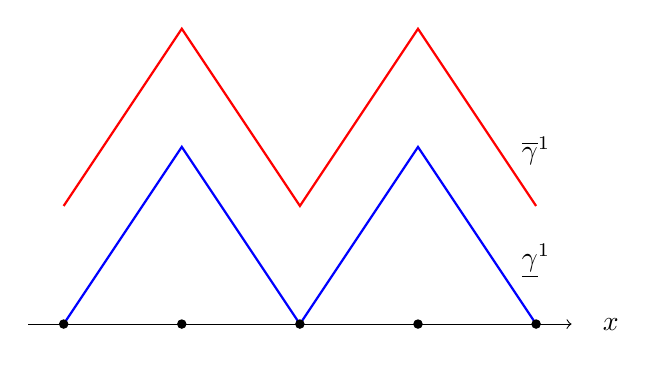
\begin{tikzpicture}[scale=1.5]
  \draw[blue,thick] (0.0,0.0) -- (1.0,1.5) -- (2.0,0.0) -- (3.0,1.5) -- (4.0,0.0)
                     node [yshift=8mm] {{\color{black} $\underline{\gamma}^1$}};
  \draw[red,thick] (0.0,1.0) -- (1.0,2.5) -- (2.0,1.0) -- (3.0,2.5) -- (4.0,1.0)
                     node [yshift=7mm] {{\color{black} $\overline{\gamma}^1$}};
  \draw[black,thin,->] (-0.3,0.0) -- (4.3,0.0) node [xshift=5mm] {$x$};
  \foreach \x in {0.0, 1.0, 2.0, 3.0, 4.0} {
      \filldraw (\x,0.0) circle (1.0pt);
  }
\end{tikzpicture}

&
\definecolor{seabornblue}{rgb}{0.2980392156862745, 0.4470588235294118, 0.6901960784313725}
\definecolor{seaborngreen}{rgb}{0.3333333333333333, 0.6588235294117647, 0.40784313725490196}
\definecolor{seabornred}{rgb}{0.7686274509803922, 0.3058823529411765, 0.3215686274509804}

\begin{tikzpicture}[scale=1.5]
  \draw[seabornblue,very thick] (0.0,1.5) -- (4.0,1.5)
                     node [xshift=-6mm,yshift=4mm] {{\color{black} $\underline{\gamma}^0 = \maxR\underline{\gamma}^1$?}};
  \draw[seabornred,very thick] (0.0,1.0) -- (4.0,1.0)
                     node [xshift=-6mm,yshift=-4mm] {{\color{black} $\overline{\gamma}^1 = \minR\overline{\gamma}^1$?}};
  \draw[black,thin,->] (-0.3,0.0) -- (4.3,0.0) node [xshift=5mm] {$x$};
  \foreach \x in {0.0, 2.0, 4.0} {
      \filldraw (\x,0.0) circle (1.5pt);
  }
\end{tikzpicture}

\end{tabular}
\caption{For the finer-level constraints $\underline{\gamma}^1$ (blue) and $\overline{\gamma}^1$ (red) on the left, direct application of $\iR,\minR,\maxR$ is problematic.  For example, if we apply the monotone injections then the resulting coarser-level constraint set $\mathcal{K}^0$ is empty because $\maxR \underline{\gamma}^1 > \minR \overline{\gamma}^1$ (right).  Defect constraints avoid this difficulty.}
\label{fig:directRbad}
\end{figure}

So suppose $w^J \in \cK^J$ is an admissible finest-level iterate for \eqref{eq:fe:vi}.  We define the \emph{finest-level defect constraints} (DCs) \cite{GraeserKornhuber2009} as the following functions in $\tilde{\mathcal{V}}^J$:
\begin{equation}
\underline{\chi}^J = \underline{\gamma}^J - w^J, \qquad \overline{\chi}^J = \overline{\gamma}^J - w^J. \label{eq:fe:defectconstraints}
\end{equation}
Definition \eqref{eq:fe:fineconstraintset} implies that $\underline{\chi}^J \le 0 \le \overline{\chi}^J$ everywhere in $\overline{\Omega}$, including on the Dirichlet boundary $\partial_D\Omega$.  If $\underline{\gamma}^J=-\infty$ then $\underline{\chi}^J=-\infty$ by definition, and similarly if $\overline{\gamma}^J=+\infty$ then $\overline{\chi}^J=+\infty$.  Observe that a corrected iterate $w^J + z^J$ is admissible, $w^J + z^J \in \cK^J$, if and only if the perturbation $z^J \in \mathcal{V}^J$ is zero on $\partial_D\Omega$ and bounded by the defect constraints, $\underline{\chi}^J \le z^J \le \overline{\chi}^J$.

Descending coarser levels, $j=J-1,\dots,1,0$, we next apply the monotone injections to generate \emph{level defect constraints} (LDCs) in $\tilde{\mathcal{V}}^j$:
\begin{equation}
\underline{\chi}^{j} = \maxR \underline{\chi}^{j+1}, \qquad \overline{\chi}^{j} = \minR \overline{\chi}^{j+1}. \label{eq:fe:chilevels}
\end{equation}
Observe that by \eqref{eq:fe:monotoneproperty} and \eqref{eq:fe:monotoneadditional},
\begin{equation}
\underline{\chi}^{J} \le \dots \le \underline{\chi}^0 \le 0 \le \overline{\chi}^0 \le \dots \le \overline{\chi}^J. \label{eq:fe:chiordering}
\end{equation}
A unilateral $J=4$ example of LDCs $\underline{\chi}^j$ is shown in Figure \ref{fig:chiphilevels}.  The LDC $\underline{\chi}^j$ is the most-negative function from $\tilde{\mathcal{V}}^j$ such that if another element of $\tilde{\mathcal{V}}^j$ is above $\underline{\chi}^j$ then it is also above $\underline{\chi}^{j+1}$; similar comments apply to $\overline{\chi}^{j}$.  Note that for Algorithm \ref{alg:fascd} below, any system satisfying \eqref{eq:fe:chiordering} will suffice; the particular formulas in \eqref{eq:fe:chilevels} are not required.

%REGENERATE using https://github.com/bueler/mg-glaciers:
%$ cd mg-glaciers/py/
%$ [modify decomposition() inside visualize.py to turn off axes and print \gamma for obstacle]
%$ ./obstacle.py -J 5 -jcoarse 1 -random -randommodes 8 -diagnostics -o defect.pdf
%fine level 5 (m=63): using 20 V(1,0) cycles -> 38.750 WU
\begin{figure}[ht]
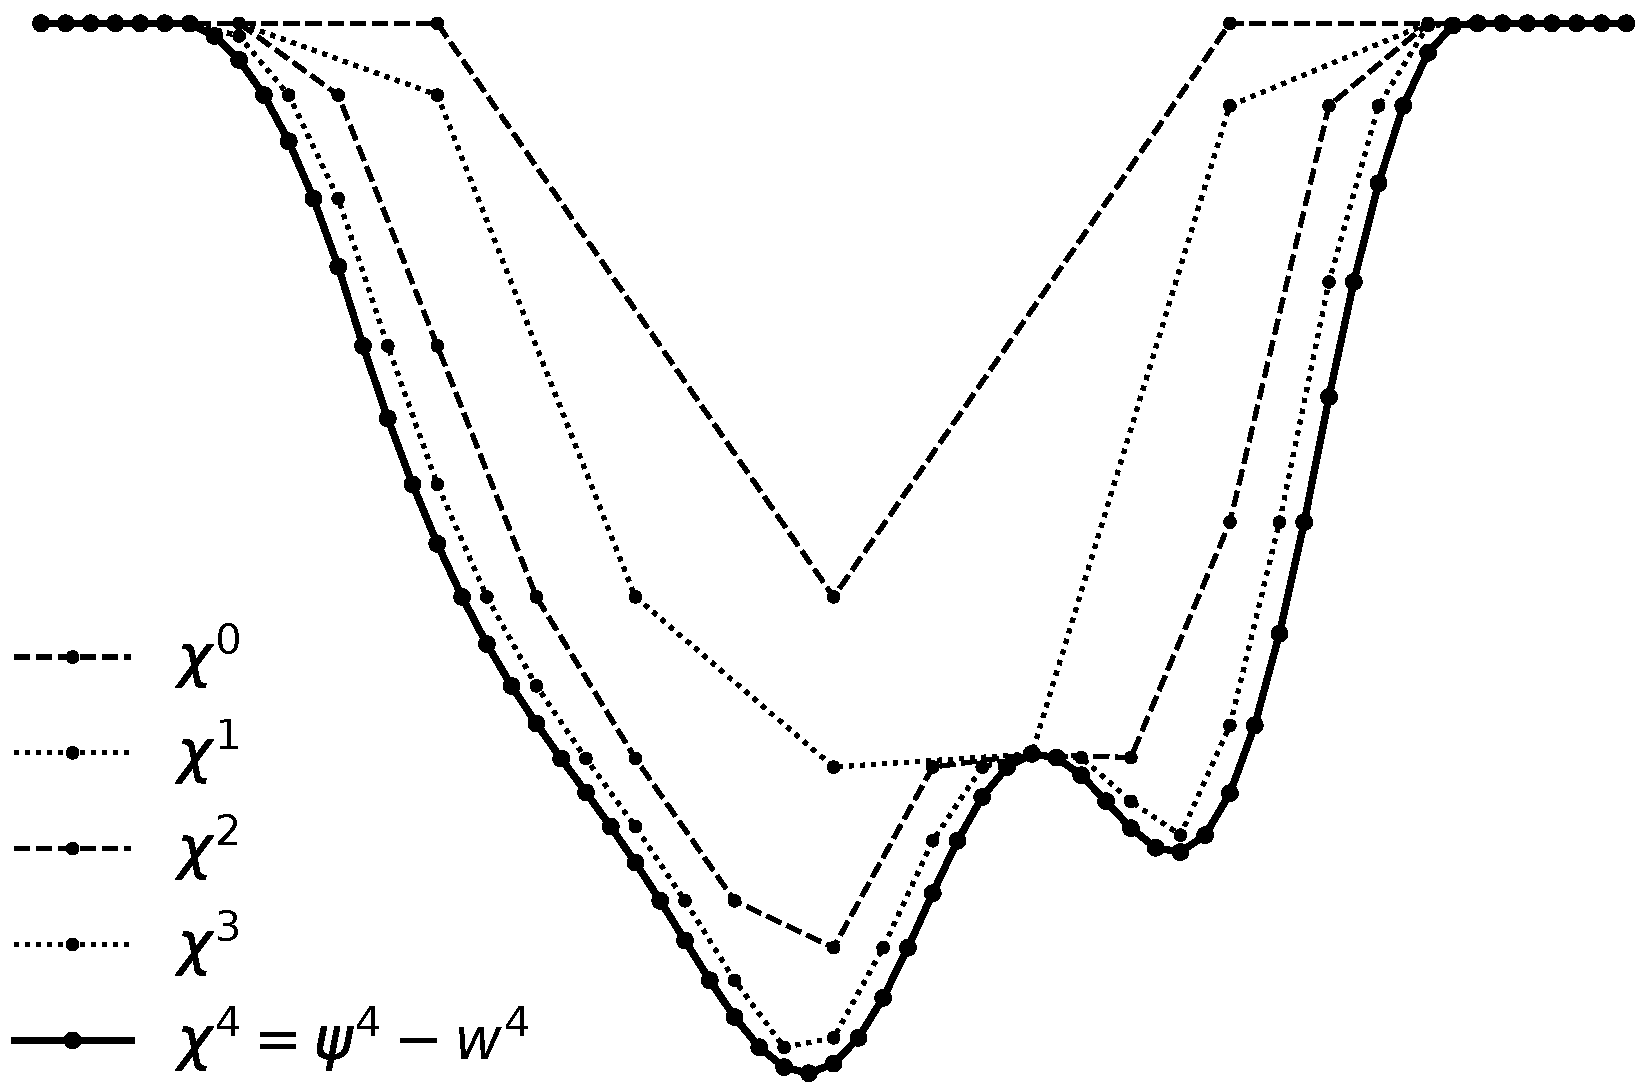
\includegraphics[width=0.65\textwidth]{fixfigs/chiphilevels.pdf}
\caption{Unilateral LDCs $\underline{\chi}^j$ are generated from $\underline{\chi}^J = \underline{\gamma}^J - w^J$ using maximum injection: $\underline{\chi}^j = \maxR \underline{\chi}^{j+1}$.}
\label{fig:chiphilevels}
\end{figure}

This construction of multilevel box constraints, as for the unilateral construction in \cite{GraeserKornhuber2009}, is designed to permit large-yet-admissible coarse corrections, which promotes multilevel solver efficiency.  However, when coarsening the problem downward in a V-cycle, one does not know what the next coarse corrections will be, and so we require constraint sets from which any sum will be admissible.  With this in mind, and looking forward to telescoping sums \eqref{eq:fe:telescoping}, we compute the LDC differences \cite{GraeserKornhuber2009}:
\begin{equation}
\underline{\phi}^j = \underline{\chi}^j - \underline{\chi}^{j-1}, \qquad \overline{\phi}^j = \overline{\chi}^j - \overline{\chi}^{j-1}.  \label{eq:fe:philevels}
\end{equation}
(Take $\underline{\chi}^{-1}=\overline{\chi}^{-1}=0$ so that $\underline{\phi}^0=\underline{\chi}^0$ and $\overline{\phi}^0=\overline{\chi}^0$.  Regarding subtraction of extended real-valued quantities, if $\underline{\chi}^j(x_p)=-\infty$ then we set $\underline{\phi}^j(x_p)=-\infty$ regardless of the value of $\underline{\chi}^{j-1}(x_p)$, and etc.)  While $\underline{\phi}^{j},\overline{\phi}^{j} \in \tilde{\mathcal{V}}^J$ again bracket zero, $\underline{\phi}^j \le 0 \le \overline{\phi}^j$, they are not ordered as in \eqref{eq:fe:chiordering}.

The corresponding \emph{downward/upward constraint sets}, respectively, are closed and convex subsets of the FE spaces $\mathcal{V}^j$:
\begin{align}
\mathcal{D}^j = \left\{v \in \mathcal{V}^j \,:\, \underline{\phi}^j \le v \le \overline{\phi}^j \text{ and } \, v|_{\partial_D\Omega} = 0\right\}, \label{eq:fe:constraintsets} \\
\mathcal{U}^j = \left\{v \in \mathcal{V}^j \,:\, \underline{\chi}^j \le v \le \overline{\chi}^j \text{ and } \, v|_{\partial_D\Omega} = 0\right\}. \notag
\end{align}
Because $\underline{\chi}^j \le \underline{\phi}^j \le 0 \le \overline{\phi}^j \le \overline{\chi}^j$, it follows that $\mathcal{D}^j \subseteq \mathcal{U}^j$.  Note that the finest-level set $\mathcal{U}^J$ is equivalent to the original constraint set $\mathcal{K}^J$: for all $z^J \in \mathcal{V}^J$,
\begin{equation}
z^J \in \mathcal{U}^J \quad \iff \quad w^J+z^J \in \mathcal{K}^J. \label{eq:fe:finestlevelequivalent}
\end{equation}

Our V-cycle solver (Algorithm \ref{alg:fascd}) will compute corrections in $\mathcal{D}^j$ for the downward stage and in $\mathcal{U}^j$ for the upward stage. This strategy is, however, based on \emph{incomplete} CDs in general box-constrained cases, as we now explain.  Each upward set $\mathcal{U}^j$ is generally only a superset of a sum of downward sets $\mathcal{D}^j$, though this becomes a true CD, i.e.~satisfying \eqref{eq:subspacedecomp}--\eqref{eq:constraintrestrictionsum}, in unilateral cases.  The following Lemma, apparently new, is based in part on the unilateral CD construction underlying Algorithm 4.7 in \cite{GraeserKornhuber2009}; see also equation (59) in \cite{Tai2003}.

\begin{lemma}  \label{lem:downwardadmissibility}  For arbitrary finest-level box constraints $\underline{\gamma}^J,\overline{\gamma}^J$ satisfying \eqref{eq:fe:boxconstraintrequirements}, it follows that
\begin{equation}
\mathcal{U}^j \supseteq \mathcal{D}^j + \mathcal{D}^{j-1} + \dots + \mathcal{D}^0 \label{eq:fe:downwardsuminclusion}
\end{equation}
for $j=0,1,\dots,J$.  In unilateral cases, where either $\underline{\gamma}^J=-\infty$ identically or $\overline{\gamma}^J=+\infty$ identically, inclusion \eqref{eq:fe:downwardsuminclusion} becomes a full CD with $\mathcal{U}^j=\sum_{i=0}^j \mathcal{D}^i$.
\end{lemma}

\begin{proof}  Subspace decomposition \eqref{eq:subspacedecomp} holds---see nesting \eqref{eq:fe:nestedspaces}---and definition \eqref{eq:fe:constraintsets} shows $\mathcal{D}^i \subset \mathcal{U}^i \subset \cV^i$.  Furthermore, telescoping sums hold for any $j=0,1,\dots,J$:
\begin{equation}
\sum_{i=0}^j \underline{\phi}^i = \underline{\chi}^j, \qquad \sum_{i=0}^j \overline{\phi}^i = \overline{\chi}^j.  \label{eq:fe:telescoping}
\end{equation}
Thus if $y^i \in \mathcal{D}^i$ for $0 \le i \le j$ then
\begin{equation}
\underline{\chi}^j = \sum_{i=0}^j \underline{\phi}^i \le \sum_{i=0}^j y^i \le \sum_{i=0}^j \overline{\phi}^i \le \overline{\chi}^j, \label{eq:fe:lemmaordering}
\end{equation}
so \eqref{eq:fe:downwardsuminclusion} holds for any box constraints.

In unilateral cases we can also construct decomposition operators $\Pi_i$ and thereby show property \eqref{eq:constraintrestrictionsum}.  For concreteness suppose $\overline{\gamma}^J=+\infty$, thus $\overline{\chi}^j=+\infty$ and $\overline{\phi}^i = +\infty$ for all levels.  For $v\in \mathcal{V}^j$ and $0\le i \le j$, let $I_{j\to i}^\ominus$ be the operator applying the minimum (monotone) injection $j-i$ times, mapping into $\mathcal{V}^i$:
\begin{equation}
I_{j\to i}^\ominus v = \minR(\dots(\minR v)\dots)  \label{eq:fe:minimummaps}
\end{equation}
(Set $I_{j\to j}^\ominus v = v$ and $I_{j\to -1}^\ominus=0$ by definition.)  Now define the following nonlinear decomposition operators $\Pi_i:\mathcal{U}^j \to \mathcal{D}^i$:
\begin{equation}
\Pi_i z^j = I_{j\to i}^\ominus(z^j - \underline{\chi}^j) - I_{j\to i-1}^\ominus(z^j - \underline{\chi}^j) + \underline{\phi}^i.  \label{eq:fe:unilateraldecompositionoperator}
\end{equation}
(Compare equation (4.9) in \cite{GraeserKornhuber2009}.)  Property \eqref{eq:fe:monotoneproperty} implies $I_{j\to i}^\ominus(z^j - \underline{\chi}^j) \ge I_{j\to i-1}^\ominus(z^j - \underline{\chi}^j)$, thus $\Pi_i z^j \ge \underline{\phi}^i$, so $\Pi_i z^j \in \mathcal{D}^i$.  On the other hand, the following sum telescopes, leaving only its first term plus the sum in \eqref{eq:fe:telescoping}:
\begin{align*}
\sum_{i=0}^j \Pi_i z^j &= z^j - \underline{\chi}^j + \sum_{i=0}^j \underline{\phi}^i = z^j.
\end{align*}
This shows \eqref{eq:constraintrestrictionsum}, thus that \eqref{eq:fe:downwardsuminclusion} is equality, yielding \eqref{eq:constraintdecomp}.  The $\underline{\gamma}^J=-\infty$ case is similar.
\end{proof}

One might attempt to convert \eqref{eq:fe:downwardsuminclusion} into a full CD for arbitrary box constraints by using decomposition maps like $\Pi_i$, for example by splitting $z^j = \min\{z^j,0\} + \max\{z^j,0\}$ and applying unilateral formulas like \eqref{eq:fe:unilateraldecompositionoperator} to $\min\{z^j,0\}$ and $\max\{z^j,0\}$ separately.  The above proof shows that the lower bound $\Pi_i (\min\{z^j,0\}) \ge \underline{\phi}^i$ indeed holds.  However, the following Example shows why $\Pi_i(\min\{z^j,0\})$ may have an arbitrarily large maximum, and thus exceed any finite upper LDC $\overline{\phi}^i$.  In fact, $\Pi_i$ does not generally map all non-positive elements of $\mathcal{U}^J$ into $\mathcal{D}^i$ if a finite upper LDC is present.  On the other hand, we can not exclude entirely-different strategies for showing full CDs in the general box-constrained case.

\begin{example}  \label{ex:notfullcd}
Let $a > 0$ be an arbitrary positive number.  Consider a 2-level hierarchy ($J=1$), and suppose the lower defect constraint is the constant function $\underline{\chi}^1=-a$.  Note $\underline{\chi}^0=\maxR \underline{\chi}^1=-a$ also, so $\underline{\phi}^1=0$ and $\underline{\phi}^0=-a$.  Suppose $z^1$ is a ``sawtooth'' function which takes on value $-a$ on the coarse vertices and value $0$ on the other vertices.  Then, for any $\overline{\chi}^1\ge 0$, we have $\overline{\chi}^1 \ge 0 \ge z^1\ge \underline{\chi}^1$, so $z^j \in \mathcal{U}^1$.  However, $I_{1\to 0}^\ominus(z^1 - \underline{\chi}^1) = \minR(z^1 - \underline{\chi}^1) = 0$ identically.  From \eqref{eq:fe:unilateraldecompositionoperator}, $\Pi_1 z^1$ simplifies to $\Pi_1 z^1 = z^1 - \underline{\chi}^1$.  But then $\Pi_1 z^1$ attains a maximum $a\ge 0$.  This maximum can be chosen to exceed any upper defect obstacle $\overline{\phi}^1$, and $\Pi_1 z^1 \notin \mathcal{D}^1$ would occur.
\end{example}

Each upward set $\mathcal{U}^j$ can also be decomposed (incompletely) down to an arbitrary coarser level.  The next Lemma, which does not follow from Lemma \ref{lem:downwardadmissibility}, justifies upward admissibility in Algorithm \ref{alg:fascd}.

\begin{lemma}  \label{lem:upwardadmissibility}  For any $j=0,1,\dots,J$ and $0\le k\le j$,
\begin{equation}
\mathcal{U}^j \supseteq \mathcal{D}^j + \mathcal{D}^{j-1} + \dots + \mathcal{D}^{k+1} + \mathcal{U}^k \label{eq:fe:upwardsuminclusion}
\end{equation}
In unilateral cases, where either $\underline{\gamma}^J=-\infty$ or $\overline{\gamma}^J=+\infty$, actually $\mathcal{U}^j = \mathcal{U}^k + \sum_{i=k+1}^j \mathcal{D}^i$. \end{lemma}

\begin{proof}  Definition \eqref{eq:fe:philevels} shows that $\underline{\chi}^j = \underline{\phi}^j + \dots + \underline{\phi}^{k+1} + \underline{\chi}^k$ and $\overline{\chi}^j = \overline{\phi}^j + \dots + \overline{\phi}^{k+1} + \overline{\chi}^k$.  If $y^i \in \mathcal{D}^i$ for $k+1 \le i \le j$ and $z^k \in \mathcal{U}^k$ then $\underline{\chi}^j \le y^j + \dots + y^{k+1} + z^k \le \overline{\chi}^j$ and \eqref{eq:fe:upwardsuminclusion}.

In unilateral cases we follow the proof of Lemma \ref{lem:downwardadmissibility}.  We can use \eqref{eq:fe:unilateraldecompositionoperator} unchanged for $i=k+1,\dots,j$, but it must be modified in the $i=k$ case: $\Pi_k z^j = I_{j\to k}^\ominus(z^j - \underline{\chi}^j) + \underline{\chi}^k$.  The remainder of the proof goes through as before.
\end{proof}

Inclusions \eqref{eq:fe:downwardsuminclusion} and \eqref{eq:fe:upwardsuminclusion}, which are special to multilevel schemes based on defect constraints, hold regardless of whether a CD operator $\Pi_i$ can be constructed.  Correspondingly, there is another basic iteration that does not need the $\Pi_i$ operators, namely an incomplete variant of \pr{cd-mult} (Section \ref{sec:cd}).  Application \pr{icd-tele} below requires $w^J\in\mathcal{K}^J$, property \eqref{eq:fe:finestlevelequivalent}, and incomplete CD \eqref{eq:fe:upwardsuminclusion}.

\begin{pseudo*}
\pr{icd-tele}(w^J)\text{:} \\+
    for $j = 0,\dots,J$: \\+
        \rm{find} $z^j\in \mathcal{U}^j$ \rm{so that for all} $v \in \mathcal{U}^j$, \\+
            $\displaystyle \ip{f\Big(w^J + \alpha \sum_{i<j} z^i + \alpha z^j\Big)}{v-z^j} \ge \ip{\ell}{v-z^j}$ \\--
    return $\tilde w^J=w^J + \alpha \sum_{i\le J} z^i$
\end{pseudo*}

While inclusions \eqref{eq:fe:downwardsuminclusion} and \eqref{eq:fe:upwardsuminclusion} suffice to show the admissibility of all iterates and corrections in Algorithm \ref{alg:fascd} below, a convergence analysis extending the arguments of \cite{GraeserKornhuber2009,Tai2003} to VIs which are not of minimization type, or to box constraints, would seem to require full CDs.


\section{FASCD V-cycle} \label{sec:vcycle}

The V-cycle applies smoothers in constraint sets $\mathcal{D}^j$ and $\mathcal{U}^j$ during the downward and upward stages, respectively.  It extends the multilevel CD schemes of Tai \cite{Tai2003} and Gr\"aser \& Kornhuber \cite[Algorithm 4.7]{GraeserKornhuber2009} by following a nonlinear full approximation scheme (FAS) approach \cite{BrandtLivne2011}, and in fact it reduces to FAS for PDEs when inequality constraints are removed (Appendix \ref{app:reductions}).

Each V-cycle generates a correction to a finest-level iterate $w^J \in \mathcal{K}^J$ by incorporating information from each coarser FE subspace $\mathcal{V}^j$.  By nesting \eqref{eq:fe:nestedspaces} these corrections all live in the fine-level subspace $\mathcal{V}^J$.\footnote{Nonetheless we use prolongation $P$ to indicate where the computer representation changes.}  The corrections are constructed, inductively, so that iterates remain admissible at every level.  Suppose $y^i \in \mathcal{D}^i$, for $i=J,\dots,j+1$, are already-computed corrections during the downward part of the V-cycle (Figure \ref{fig:fascdvcycle}).  By \eqref{eq:fe:downwardsuminclusion} the correction at this point is admissible, namely $y^J + \dots + y^{j+1} \in \mathcal{U}^J$, equivalently $w^J + y^J + \dots + y^{j+1} \in \mathcal{K}^J$.  Smoothing then occurs at the next-coarser level, yielding the next correction $y^j \in \mathcal{D}^j$.  Solving the coarsest-level VI results in the full downward correction $y^J + \dots + y^1 + z^0 \in \mathcal{U}^J$.  Starting upward, $y^1 + z^0 \in \mathcal{U}^1$ is an initial iterate for smoothing on level $j=1$, which then yields $z^1 \in \mathcal{U}^1$ and an admissible correction $y^J + \dots + y^2 + z^1 \in \mathcal{U}^J$, using \eqref{eq:fe:upwardsuminclusion}.  Continuing in this ``telescoping'' way, up-smoothing in the constraint sets $\mathcal{U}^j$, starting from initial iterate $y^j+z^{j-1}$, finally generates $z^J\in \mathcal{U}^J$ as the V-cycle correction.  Then the corrected finest-level iterate is $\tilde{w}^J = w^J + z^J \in \mathcal{K}^J$.

\begin{figure}[ht]
\begin{center}
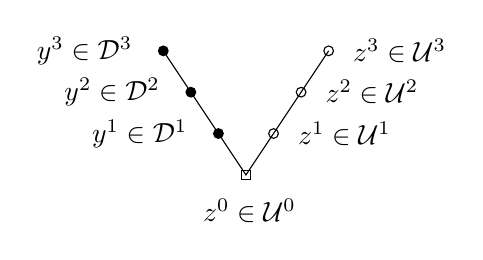
\begin{tikzpicture}[scale=0.7]
  \pgfmathsetmacro\hstep{0.5}
  \pgfmathsetmacro\vstep{0.75}
  \pgfmathsetmacro\ceps{0.08}   % size of square for coarse grid

% V-cycle with MCD down-obstacle and up-obstacle annotations
  \draw[black,thin] (-\hstep,3*\vstep) -- (0.0,2*\vstep) -- (\hstep,\vstep) --  (2*\hstep,0.0)
                    -- (3*\hstep,\vstep) -- (4*\hstep,2*\vstep) -- (5*\hstep,3*\vstep);
  \filldraw (-\hstep,3*\vstep) node[xshift=-10mm] {$y^3 \in \mathcal{D}^3$} circle (2.5pt);
  \filldraw (0.0,2*\vstep) node[xshift=-10mm] {$y^2 \in \mathcal{D}^2$} circle (2.5pt);
  \filldraw (\hstep,\vstep) node[xshift=-10mm] {$y^1 \in \mathcal{D}^1$} circle (2.5pt);
  \draw     (2*\hstep-\ceps,-\ceps) node[xshift=1mm,yshift=-4mm] {$z^0 \in \mathcal{U}^0$} rectangle (2*\hstep+\ceps,+\ceps);
  \draw     (3*\hstep,\vstep) node[xshift=9mm] {$z^1 \in \mathcal{U}^1$} circle (2.5pt);
  \draw     (4*\hstep,2*\vstep) node[xshift=9mm] {$z^2 \in \mathcal{U}^2$} circle (2.5pt);
  \draw     (5*\hstep,3*\vstep) node[xshift=9mm] {$z^3 \in \mathcal{U}^3$} circle (2.5pt);
\end{tikzpicture}

\end{center}
\caption{The FASCD V-cycle computes downward corrections $y_j \in \mathcal{D}^j$, but the upward corrections $z_j\in\mathcal{U}^j$ are in larger sets.}
\label{fig:fascdvcycle}
\end{figure}

A key idea is that, because of inclusions \eqref{eq:fe:upwardsuminclusion}, up-smoothing solves less-restricted VI problems than down-smoothing.  Intuitively-speaking, going downward one does not know what the next coarse corrections will be, and thus on any level one must choose conservative constraint sets $\mathcal{D}^j$ so that the sum of the corrections is admissible once we return to a given level.  Going upward, however, no further coarse corrections can violate admissibility.

To state the V-cycle algorithm below we must also clarify the problems solved at each mesh level.  As in FAS multigrid for nonlinear PDEs \cite{BrandtLivne2011,Bruneetal2015,Trottenbergetal2001}, both the solution approximation and the residual must be coarsened, and a source functional created.  On mesh level $j$ we assume a re-discretized nonlinear operator $f^j$, with output in $(\cV^j)'$, which is an FE discretization of $f$ in \eqref{eq:boxdirichletvi}.\footnote{Presumably it uses quadrature etc.~in the same scheme which generated $f^J$ in \eqref{eq:fe:vi}.}  Finally, we assume that an admissible iterate $w^J \in \mathcal{K}^J$ has already\footnote{In practice the LDCs $\underline{\chi}^j,\overline{\chi}^j,\underline{\phi}^j,\overline{\phi}^j$ are generated during the descent stage; see Algorithm \ref{alg:fascd}.} been used to generate the LDCs and constraint sets $\mathcal{D}^j$, $\mathcal{U}^j$ at each level (Section \ref{sec:cdmultilevel}); these LDCs do not depend on the coarse-level corrections.

As we descend we define new $j$th-level iterates
\begin{equation}
w^j = \iR(w^{j+1} + y^{j+1}).  \label{eq:fe:definew}
\end{equation}
(These are the states before smoothing or correction.)  From $w^j$ we define $\ell^j \in (\cV^j)'$:
\begin{equation}
\ell^j = \begin{cases} \ell^J, & j=J \\
                       f^j(w^j) + R\left(\ell^{j+1}-f^{j+1}(w^{j+1}+y^{j+1})\right), & j<J. \end{cases} \label{eq:fe:levelsource}
\end{equation}
Observe that injection $\iR$ coarsens the (primal) iterates---injection is commonly used in classical FAS \cite[section 5.3]{Trottenbergetal2001}---but canonical restriction $R$ coarsens (dual) linear functionals; recall Table \ref{tab:transfers}.  On descent, at levels $j=J,J-1,\dots,1$, we solve the following VI for $y^j \in \mathcal{D}^j$:
\begin{equation}
\ip{f^j(w^j + y^j)}{v-y^j} \ge \ip{\ell^j}{v-y^j} \qquad \text{for all } v\in \mathcal{D}^j, \label{eq:fe:downvi}
\end{equation}
for which the initial iterate is $y_{(0)}^j=0$.  (Zero is admissible; see the comment after \eqref{eq:fe:philevels}.)

On ascent, $j=0,1,\dots,J$, the same VI is solved but for $z^j \in \mathcal{U}^j$:
\begin{equation}
\ip{f^j(w^j + z^j)}{v-z^j} \ge \ip{\ell^j}{v-z^j} \qquad \text{for all } v\in \mathcal{U}^j. \label{eq:fe:upvi}
\end{equation}
The nontrivial initial iterate for this problem is found by prolonging $z^{j-1}$ and using it to correct the current (i.e.~down-smoothed) correction on the level:
\begin{equation}
z_{(0)}^j = y^j + P z^{j-1}.  \label{eq:fe:upwardinitial}
\end{equation}
An exception is that $z_{(0)}^0=0$ on the coarsest level.  Note $z_{(0)}^j$ is admissible by \eqref{eq:fe:upwardsuminclusion}.

%If we were to inject the original box constraints \eqref{eq:fe:fineconstraintset} downward to coarser meshes, i.e.~$\underline{\gamma}^j = \iR \underline{\gamma}^{j+1}$ and $\overline{\gamma}^j = \iR \overline{\gamma}^{j+1}$, then, because injection preserves inequalities, and because $y^{j+1} \in \mathcal{D}^{j+1}$, it would follow from \eqref{eq:fe:definew} that $\underline{\gamma}^j \le w^j \le \overline{\gamma}^j$.  In this sense $w^j$ is admissible with respect to the box constraints.  However, while $w^j \in \cV^j \subset \cV^J$ holds, generally $w^j \notin \cK^J$, and furthermore our use of LDCs (Section \ref{sec:cdmultilevel}) avoids the need to generate these $\underline{\gamma}^j, \overline{\gamma}^j$.

Observe that formula \eqref{eq:fe:levelsource} for functional $\ell^j$ is a classical FAS construction for PDEs; compare equation (8.5b) in \cite{BrandtLivne2011} or equation (5.3.14) in \cite{Trottenbergetal2001}.  It has the following explanation, which simultaneously justifies VI problems \eqref{eq:fe:downvi} and \eqref{eq:fe:upvi}.  First, the $j+1$ level problem \eqref{eq:fe:downvi} is not solved exactly by the finer-level correction $y^{j+1}$---the down-smoother was only approximate---so we seek a further correction $y$ on the $j+1$ level such that
\begin{equation}
\ip{f^{j+1}(w^{j+1}+y^{j+1}+y)}{v-y^{j+1}-y} \ge \ip{\ell^{j+1}}{v-y^{j+1}-y} \quad \text{\emph{(notional)}} \label{eq:fe:downvinotional}
\end{equation}
for all $v\in \mathcal{D}^j$.  However, in fact $y$ will be approximated by solving a coarser, $j$th-level problem generated by modifying \eqref{eq:fe:downvinotional} in 4 steps:
\begin{enumerate}
\item subtract the computable quantity $f^{j+1}(w^{j+1}+y^{j+1}) \in (\mathcal{V}^{j+1})'$ from both sides,
\item replace the residual $\ell^{j+1}-f^{j+1}(w^{j+1}+y^{j+1})$ on the right by its restriction,
\item replace $w^{j+1}+y^{j+1}$, where it appears on the left, by its injection, and
\item where it appears on the left, replace $f^{j+1}$ by the coarser rediscretization $f^j$.
\end{enumerate}
Steps \emph{(ii)}--\emph{(iv)} are justified when the residual and the error are smooth; such smoothness should result from application of the down-smoother.  These steps yield a problem for the $j$th-level correction $y^j \in \mathcal{D}^j$:
\begin{align}
&\ip{f^j\left(\iR(w^{j+1}+y^{j+1})+y^j\right)}{v-y^j} - \ip{f^j\left(\iR(w^{j+1}+y^{j+1})\right)}{v-y^j} \label{eq:fe:downvicluttered} \\
&\qquad \ge \ip{R\left(\ell^{j+1}-f^{j+1}(w^{j+1}+y^{j+1})\right)}{v-y^j} \notag
\end{align}
This is the same as VI problem \eqref{eq:fe:downvi}, but in cluttered form, motivating definitions \eqref{eq:fe:definew} and \eqref{eq:fe:levelsource}.  The explanation for VI \eqref{eq:fe:upvi} is similar.

These ideas come together in Algorithm \ref{alg:fascd}, \pr{fascd-vcycle}, which updates $w^J$.  It assumes that the \pr{smooth} and \pr{solve} procedures do in-place modifications of their final arguments, without modifying their first four arguments.  Parameters \id{down} and \id{up} determine the number of smoother iterations, respectively.

\begin{pseudofloat}[ht]
\begin{pseudo}
\pr{fascd-vcycle}(J,\ell^J,\underline{\gamma}^J,\overline{\gamma}^J;w^J)\text{:} \\+
    $\underline{\chi}^J, \, \overline{\chi}^J = \underline{\gamma}^J - w^J, \, \overline{\gamma}^J - w^J {\large \strut}$ \label{line:vcyclegenchifinest} \\
    for $j=J$ downto $j=1$ \\+
      $\underline{\chi}^{j-1}, \, \overline{\chi}^{j-1} = \maxR \underline{\chi}^j, \, \minR \overline{\chi}^j {\large \strut}$ \label{line:vcyclegenchi} \\
      $\underline{\phi}^j, \, \overline{\phi}^j = \underline{\chi}^j - P\underline{\chi}^{j-1}, \, \overline{\chi}^j - P\overline{\chi}^{j-1} {\large \strut}$ \label{line:vcyclegenphi} \\
      $y^j = 0$ \\
      $\text{\pr{smooth}}^{\text{\id{down}}}(\ell^j,\underline{\phi}^j,\overline{\phi}^j,w^j;y^j)$  \ct{smoothing of \eqref{eq:fe:downvi} in $\mathcal{D}^j$}\\
      $w^{j-1} = \iR(w^j + y^j)$ \label{line:vcyclerestrictsolution} \\
      $\ell^{j-1} = f^{j-1}(w^{j-1}) + R \left(\ell^j - f^j(w^j+y^j)\right)$ \label{line:vcyclerestrictell} \\-
    $z^0 = 0$ \\
    $\text{\pr{solve}}(\ell^0,\underline{\chi}^0,\overline{\chi}^0,w^0;z^0)$ \hspace{1.0cm} \ct{solving of \eqref{eq:fe:upvi} in $\mathcal{U}^0$} \\
    for $j=1$ to $j=J$ \\+
      $z^j = y^{j} + P z^{j-1}$ \label{line:vcycleupsmoothinitial} \\
      $\text{\pr{smooth}}^{\text{\id{up}}}(\ell^j,\underline{\chi}^j,\overline{\chi}^j,w^j;z^j)$  \ct{smoothing of \eqref{eq:fe:upvi} in $\mathcal{U}^j$} \\-
    return $w^J+z^J$
\end{pseudo}
\caption{The FASCD V-cycle is an iteration for solving VI problem \eqref{eq:fe:vi}.  Here $f^j$ denotes an FE discretization of $f$ in problem \eqref{eq:boxdirichletvi}.}
\label{alg:fascd}
\end{pseudofloat}

Algorithm \ref{alg:fascd} is a $V(1,1)$ cycle with \id{down}, \id{up} smoother iterations on each level.  For \id{up} $=0$ it becomes a $V(1,0)$ cycle, and for \id{down} $=0$ a $V(0,1)$ cycle.  The $V(1,0)$ cycle is similar to Algorithm 4.7 in \cite{GraeserKornhuber2009}, but generalizes it by applying FAS-type corrections and allowing any smoother or nonlinear operator $f$.  One iteration of \pr{fascd-vcycle} is an application of \pr{cd-mult} (Section \ref{sec:cd}) over CD\footnote{Strictly speaking, this statement is restricted to unilateral cases.} \eqref{eq:fe:downwardsuminclusion} followed by an application of \pr{icd-tele} (Section \ref{sec:cdmultilevel}) over incomplete CD \eqref{eq:fe:upwardsuminclusion}, and in this sense $V(1,1)=V(1,0)+V(0,1)$.

Regarding the storage required, let us assume all box constraints are nontrivial. In this case, seven vectors must be allocated on each level: $\underline{\chi}^j$, $\overline{\chi}^j$, $\underline{\phi}^j$, $\overline{\phi}^j$, $w^j$, $\ell^j$, $y^j$.  Note $z^j$ can use the same storage as $y^j$.  On the finest level one must also store $\underline{\gamma}^J$ and $\overline{\gamma}^J$, while on the coarsest level there are only five vectors because $\underline{\phi}^0=\underline{\chi}^0$ and $\overline{\phi}^0=\overline{\chi}^0$.  Therefore, using $m_j=2^d m_{j-1}$, plus a geometric series argument, the total storage, excluding smoother and coarse-solver implementations, is
\begin{equation}
9 m_J + 7 m_{J-1} + \dots + 7 m_1 + 5 m_0 \le \left(9 + \frac{7}{2^d - 1}\right) m_J.
\end{equation}
This gives storage at most $16m_J$, $12m_J$, and $10m_J$ in dimensions $d=1,2,3$, respectively.  For comparison, a single-level method needs $4 m_J$ storage (i.e.~$\underline{\gamma}^J,\overline{\gamma}^J,\ell^J,w^J$).  If some of the obstacles are trivial, for instance in the unilateral case $\overline{\gamma}^J=+\infty$, storage can be correspondingly reduced at all levels.


\section{Implementation} \label{sec:implementation}

Implementations of FASCD methods must choose a concrete convergence criterion.  In this section we also construct the F-cycle extension, and we describe the active set Newton method we will use as a smoother and coarse solver.

Because the problem is inequality-constrained, repeated application of Algorithm \ref{alg:fascd} to solve the finite-dimensional, box-constrained VI \eqref{eq:fe:vi} will not generally reduce the residual $f^J(w^J) - \ell^J$ to zero everywhere.  To construct appropriate convergence criteria for the discretization, note \eqref{eq:fe:vi} is equivalent to a \emph{mixed complementarity problem} (MCP) \cite{FacchineiPang2003}.  By definition, this says that certain node-wise conditions hold for $u^J$ at $x_p \in \mathcal{T}^J$.  Let $r(u^J)_p = \ip{f^J(w^J)-\ell^J}{\psi_p}$ be the pointwise (ordinary) residual.  If $x_p \notin \partial_D\Omega$ then one of these four conditions must hold:
\begin{itemize}
\item $\underline{\gamma}^J(x_p)<u^J(x_p)<\overline{\gamma}^J(x_p)$ and $r(u^J)_p = 0$,
\item $\underline{\gamma}^J(x_p)=u^J(x_p)<\overline{\gamma}^J(x_p)$ and $r(u^J)_p \ge 0$,
\item $\underline{\gamma}^J(x_p)<u^J(x_p)=\overline{\gamma}^J(x_p)$ and $r(u^J)_p \le 0$,
\item $\underline{\gamma}^J(x_p)=u^J(x_p)=\overline{\gamma}^J(x_p)$.
\end{itemize}
Otherwise, if $x_p \in \partial_D\Omega$ then
\begin{itemize}
\item $u^J(x_p)=g_D^J(x_p)$.
\end{itemize}
These five cases might be labeled \emph{inactive}, \emph{lower active}, \emph{upper active}, \emph{pinched} (\emph{both active}), and \emph{boundary}, respectively.  Where \emph{pinched} or \emph{boundary} apply, $r(u^J)_p$ can have any value.

This MCP interpretation allows us to construct expressions whose norms should approach zero.  For $w^J \in \mathcal{K}^J$ we define the finest-level \emph{nodal complementarity residual} $\rNC(w^J)$ from the five cases:
\begin{equation}
\rNC(w^J)_p = \begin{cases}
    r(w^J)_p, & \underline{\gamma}^J(x_p) < w^J(x_p) < \overline{\gamma}^J(x_p), \\
    \min\{r(w^J)_p,0\}, & w^J(x_p) = \underline{\gamma}^J(x_p), \\
    \max\{r(w^J)_p,0\}, & w^J(x_p) = \overline{\gamma}^J(x_p), \\
    0, & \underline{\gamma}^J(x_p)=w^J(x_p)=\overline{\gamma}^J(x_p), \\
    w^J(x_p) - g_D^J(x_p), & x_p \in \partial_D\Omega. \end{cases} \label{eq:rNC}
\end{equation}
The first four cases assume $x_p \notin \partial_D\Omega$.  For PDEs one uses only the first and last cases.

The computable nonlinear map $\rNC : \mathcal{K}^J \to \RR^{m_J}$ in \eqref{eq:rNC} is defined using only the finest-level objects $f^J,\ell^J,\underline{\gamma}^J,\overline{\gamma}^J$.  A value $\rNC(w^J)_p$ is nonzero only at vertices where the MCP is violated, and the formula applies as stated if $\underline{\gamma}^J(x_p)=-\infty$ or $\overline{\gamma}^J(x_p)=+\infty$.  However, direct implementation of \eqref{eq:rNC} is sensitive to rounding error because $\rNC$ is a discontinuous function of $w^J(x_p)$.  For example, if $w^J(x_p)$ exceeds $\underline{\gamma}^J(x_p)$ by $10^{-16}$, then evaluation of $\rNC$ would falsely suggest that the iteration is far from converging.  Thus we instead measure convergence using the Fischer-Burmeister function \cite{BensonMunson2006,Ulbrich2011} on $a,b\in\RR$:
\begin{equation}
\phi(a,b) = a + b - \sqrt{a^2 + b^2}. \label{eq:phiFB}
\end{equation}
Observe that $\phi$ is semi-smooth, thus continuous, and that $\phi(a,b)=0$ if and only if $a,b$ are complementary.  For convenience denote $\underline{g}_p = w^J(x_p) - \underline{\gamma}^J(x_p)$ and $\overline{g}_p = \overline{\gamma}^J(x_p) - w^J(x_p)$, the nonnegative gaps at $x_p$.  Now define the \emph{semi-smooth residual}
\begin{equation}
\rSS(w^J)_p = \begin{cases}
\max\big\{\phi\big(\underline{g}_p, r(w^J)_p\big), \phi\left(\overline{g}_p, -r(w^J)_p\right)\big\}, & x_p \notin \partial_D\Omega, \\
w^J(x_p) - g_D^J(x_p), & x_p \in \partial_D\Omega.
\end{cases} \label{eq:rSS}
\end{equation}
Straightforward modifications apply for unconstrained degrees of freedom, where $\overline{\gamma}^J(x_p) = +\infty$ or $\underline{\gamma}^J(x_p) = -\infty$ or both.

Suppose an iteration starts with $w^{J,0} \in \mathcal{K}^J$, generating (fine-level) iterates $w^{J,k} \in \mathcal{K}^J$.  Let $\id{atol}\ge 0$, $\id{rtol}\ge 0$ be given tolerances.  We employ
\begin{equation}
\|\rSS(w^{J,k})\|_2 < \id{atol} \qquad \text{or} \qquad \frac{\|\rSS(w^{J,k})\|_2}{\|\rSS(w^{J,0})\|_2} < \id{rtol} \label{eq:stoppingcriterion}
\end{equation}
as the stopping criterion.  In Section \ref{sec:results} we will show that iteration of the V-cycle Algorithm \ref{alg:fascd}, starting with some finest-mesh initial iterate $w^{J,0}$ and repeated until \eqref{eq:stoppingcriterion} holds, is an effective solver.

However, an F-cycle (Figure \ref{fig:fcycle}), also called a \emph{full multigrid cycle}, is even better.  The well-known principle of such a cycle \cite[section 2.6]{Trottenbergetal2001} is to start on the coarsest mesh and solve the problem from any initial iterate.  Then an admissible initial iterate on the next-finer mesh is generated via prolongation, and so on to finer levels.  (In the VI context one must also truncate to the bounds after the prolongation; see lines \ref{line:fcycleprolongtruncone} and \ref{line:fcycleprolongtrunctwo} in Algorithm \ref{alg:fascd-fcycle}.)  During this ``ramp'' one approximately solves on each level by using a fixed number of V-cycles, each down to the coarsest mesh, and then one does full-depth V-cycles from the finest level, to convergence.

\begin{figure}[h]
\begin{center}
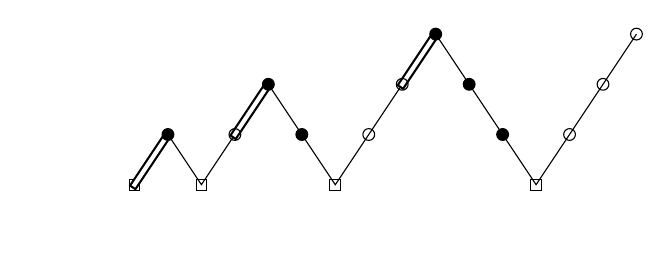
\begin{tikzpicture}[scale=0.85]
  \pgfmathsetmacro\hstep{0.5}
  \pgfmathsetmacro\vstep{0.75}
  \pgfmathsetmacro\ceps{0.08}   % size of square for coarse grid

% initial restriction to coarsest
  \pgfmathsetmacro\hoff{0*\hstep}
  %\draw[shift={(\hoff,0)},gray,line width=1.0mm] (0.0,3*\vstep) -- (\hstep,2*\vstep) --  (2*\hstep,\vstep) -- (3*\hstep,0.0);
  \draw[shift={(\hoff,0)}]     (3*\hstep-\ceps,-\ceps) rectangle (3*\hstep+\ceps,+\ceps);
  \draw[shift={(\hoff,0)},black,thick,double,double distance between line centers=0.8mm,line cap=rect] (3*\hstep,0.0) -- (4*\hstep,\vstep);

% V-cycle to level 1
  \pgfmathsetmacro\hoff{4*\hstep}
  \draw[shift={(\hoff,0)},black,thin] (0.0,\vstep) -- (\hstep,0.0) -- (2*\hstep,\vstep);
  \draw[shift={(\hoff,0)},black,thick,double,double distance between line centers=0.8mm,line cap=rect] (2*\hstep,\vstep) -- (3*\hstep,2*\vstep);
  \filldraw[shift={(\hoff,0)}] (0.0,\vstep) circle (2.5pt);
  \draw[shift={(\hoff,0)}]     (\hstep-\ceps,-\ceps) rectangle (\hstep+\ceps,+\ceps);
  \draw[shift={(\hoff,0)}]     (2*\hstep,\vstep) circle (2.5pt);

% V-cycle to level 2
  \pgfmathsetmacro\hoff{7*\hstep}
  \draw[shift={(\hoff,0)},black,thin] (0.0,2*\vstep) --  (\hstep,\vstep) -- (2*\hstep,0.0) -- (3*\hstep,\vstep) -- (4*\hstep,2*\vstep);
  \draw[shift={(\hoff,0)},black,thick,double,double distance between line centers=0.8mm,line cap=rect] (4*\hstep,2*\vstep) -- (5*\hstep,3*\vstep);
  \filldraw[shift={(\hoff,0)}] (0.0,2*\vstep) circle (2.5pt);
  \filldraw[shift={(\hoff,0)}] (\hstep,\vstep) circle (2.5pt);
  \draw[shift={(\hoff,0)}]     (2*\hstep-\ceps,-\ceps) rectangle (2*\hstep+\ceps,+\ceps);
  \draw[shift={(\hoff,0)}]     (3*\hstep,\vstep) circle (2.5pt);
  \draw[shift={(\hoff,0)}]     (4*\hstep,2*\vstep) circle (2.5pt);

% V-cycle to finest (level 3)
  \pgfmathsetmacro\hoff{12*\hstep}
  \draw[shift={(\hoff,0)},black,thin] (0.0,3*\vstep) -- (\hstep,2*\vstep) --  (2*\hstep,\vstep) -- (3*\hstep,0.0) -- (4*\hstep,\vstep) -- (5*\hstep,2*\vstep) -- (6*\hstep,3*\vstep);
  \filldraw[shift={(\hoff,0)}] (0.0,3*\vstep) circle (2.5pt);
  \filldraw[shift={(\hoff,0)}] (\hstep,2*\vstep) circle (2.5pt);
  \filldraw[shift={(\hoff,0)}] (2*\hstep,\vstep) circle (2.5pt);
  \draw[shift={(\hoff,0)}]     (3*\hstep-\ceps,-\ceps) rectangle (3*\hstep+\ceps,+\ceps);
  \draw[shift={(\hoff,0)}]     (4*\hstep,\vstep) circle (2.5pt);
  \draw[shift={(\hoff,0)}]     (5*\hstep,2*\vstep) circle (2.5pt);
  \draw[shift={(\hoff,0)}]     (6*\hstep,3*\vstep) circle (2.5pt);

  \draw[white] (0, -\vstep) circle (2.5pt);
\end{tikzpicture}


\end{center}
\caption{F-cycle Algorithm \ref{alg:fascd-fcycle} initially restricts and injects the data $\ell^J,\underline{\gamma}^J,\overline{\gamma}^J$ down to level $j=0$ (gray).  Then it prolongs and truncates (doubled edges) to create an admissible initial iterate on the next-finer level.  Solution on each level is by V-cycles. See Figure \ref{fig:fascdvcycle} for the other symbols.}
\label{fig:fcycle}
\end{figure}

This F-cycle approach is described in Algorithm \ref{alg:fascd-fcycle}.  In contrast to the construction of LDCs (Section \ref{sec:cdmultilevel}) for V-cycles, standard injection is used to generate the $\underline{\gamma}^j,\overline{\gamma}^j$ on each level during the initial nested iteration. This is because nested iteration approximates the full solution on the coarse grids, not just a correction to an initial iterate; essentially, our choice is between \eqref{eq:fe:badstandard} (where the coarse constraint set is always nonempty, but the solution may not be admissible on the next level) or \eqref{eq:fe:badmonotone} (where the coarse solution is always admissible if it exists, but the constraint set may be empty). We choose \eqref{eq:fe:badstandard} so that the coarse problems always have nonempty constraint sets, and project pointwise to the bounds as we refine in the nested iteration.
On line \ref{line:fcyclecoarsestinitial}, one may generate an initial iterate $w^0\in\mathcal{K}^0$ by injection and truncation of a finest-level iterate, if one is available.

\begin{pseudofloat}[h]
\begin{pseudo}
\pr{fascd-fcycle}(J,\ell^J,\underline{\gamma}^J,\overline{\gamma}^J)\text{:} \\+
    for $j=J$ downto $j=1$ \\+
        $\ell^{j-1} = R(\ell^j)$ \\
        $\underline{\gamma}^{j-1}, \, \overline{\gamma}^{j-1} = \iR \underline{\gamma}^{j}, \, \iR \overline{\gamma}^{j}$ {\large\strut} \\-
    choose $w^0 \in \mathcal{K}^0$ \label{line:fcyclecoarsestinitial} \\
    $\text{\pr{solve}}(\ell^0,\underline{\gamma}^0,\overline{\gamma}^0;w^0)$ \\
    for $j=1$ to $j=J-1$ \\+
        $w^j = \max\left\{\underline{\gamma}^{j},\min\{\overline{\gamma}^{j}, Pw^{j-1}\}\right\} \in \mathcal{K}^j$ \label{line:fcycleprolongtruncone} \\
        $\pr{fascd-vcycle}^{\text{\id{rampv}}}(j,\ell^j,\underline{\gamma}^j,\overline{\gamma}^j;w^j)$ \\-
    $w^J = \max\left\{\underline{\gamma}^{J},\min\{\overline{\gamma}^{J}, Pw^{J-1}\}\right\} \in \mathcal{K}^J$ \label{line:fcycleprolongtrunctwo} \\
    while not \eqref{eq:stoppingcriterion} \\+
        \pr{fascd-vcycle}(J,\ell^J,\underline{\gamma}^J,\overline{\gamma}^J;w^J) \\-
    return $w^J$
\end{pseudo}
\caption{The FASCD F-cycle for solving VI problem \eqref{eq:fe:vi}.}
\label{alg:fascd-fcycle}
\end{pseudofloat}

\begin{comment}
smoother semantics: in our implementation of the V-cycle we actually shift to solve a VI for $\tilde w^j = w^j+y^j$, then compute $y^j = \tilde w^j - w^j$ after the solve, etc.; this is evidently equivalent
\end{comment}

A large space of smoothers could be explored, but in Section \ref{sec:results} we apply a fixed number of iterations of the active-set (reduced-space) Newton method from \cite{BensonMunson2006}, the \texttt{VINEWTONRSLS} solver in PETSc \cite{Balayetal2023}, denoted as \emph{RS Newton}.  A fixed number of preconditioned Krylov iterations are applied to approximately solve the arising linear systems.  For the symmetric Laplacian in Example \ref{ex:results:classical} we apply conjugate gradients (CG) with incomplete Cholesky (IC) preconditioning, but for other operators we apply the generalized minimum residual (GMRES) method with incomplete LU (ILU) preconditioning.  This smoother requires $O(m_j)$ work per iteration. The coarse solver is also RS Newton, but iterated to convergence, with a direct solver for the arising linear systems.


\section{Results} \label{sec:results}

Algorithms \ref{alg:fascd} and \ref{alg:fascd-fcycle} were implemented in Python, for $P_1$ and $Q_1$ elements, using the Firedrake library \cite{Rathgeberetal2016}.  Here we show numerical results for the example problems presented in Section \ref{sec:vi}, with a focus on the scaling of FASCD iterations as the mesh resolution increases.  Our primary observations are that each V-cycle greatly reduces the residual norm, and that very few F-cycles solve most examples to within discretization error.

\begin{example} \label{ex:results:classical}
Consider the unilateral 2D Laplacian obstacle problem, Example \ref{ex:plaplacian} with $p=2$ and admissible set $\mathcal{K} = \{v \ge \psi\} \subset W^{1,2}(\Omega)$.  We consider two problems, both over square domains $\Omega$, with the very different coincidence (active) sets $\{x\in\Omega \,:\, u(x)=\psi(x)\}$ shown in Figure \ref{fig:results:classical}.  The standard ``ball'' problem has an upper hemisphere obstacle $\psi$ \cite[Chapter 12]{Bueler2021}.  For the ``spiral'' problem \cite[problem 7.1.1]{GraeserKornhuber2009}, $\psi$ is constructed to produce the coincidence set shown.  For this experiment we used a coarsest regular-triangulation mesh with $m_0=5^2$ vertices (32 triangles).  The finest mesh, built by standard refinement, had $m_9=2049^2 \approx 4.2 \times 10^{6}$ vertices.  As our smoother we applied a single RS Newton iteration (Section \ref{sec:implementation}), with three (fixed) IC-preconditioned CG iterations to approximately solve the arising linear systems.  The coarse solver was RS$+$LU, iterated to convergence.  Tolerances \texttt{rtol} $= 10^{-6}$ and \texttt{atol} $= 10^{-12}$ were used in stopping criterion \eqref{eq:stoppingcriterion}.  The initial iterate was set to $w=\max\{0,\psi\}$.

Table \ref{tab:results:classical} shows the resulting iteration counts.  When the RS Newton smoother is applied by itself as a solver (``RS only''), as expected it shows rapidly-increasing iterations, roughly proportional to resolution.  By contrast, V-cycle iterations increase slowly, perhaps logarithmically with the resolution.  For F-cycles we report the number of V-cycles after the ramp (Section \ref{sec:implementation}); a constant number solves the problem.  Comparing the ball and spiral results, the complexity of the coincidence set or free boundary does not appear to strongly influence FASCD performance.  For the spiral results, note that \cite{GraeserKornhuber2009} reports more than 30 iterations of all their tested methods were required to achieve similar tolerance for $m_J \approx 5\times 10^5$.

Each V-cycle does the work of about eight finest-level preconditioned Krylov (CG+IC) iterations.  Thus for the F-cycle results, where three iterations suffice at all resolutions, we see close to textbook multigrid efficiency\footnote{Textbook multigrid efficiency is imperfectly defined, but consider \cite{BrownSmithAhmadia2013}: ``an order of magnitude reduction in residual per iteration and solution of the fine-level system at a small multiple of the cost of a residual evaluation.''  Work of less than ten residual evaluations is often mentioned as the standard.} despite the low solution regularity.
\end{example}

%REGENERATE using git@bitbucket.org:pefarrell/fascd.git, in examples/
%$ python3 drape.py -prob ball -levs 9 -o ball -fascd_rtol 1.0e-6 -fascd_atol 1.0e-6 -fascd_cycle_type full
%$ mpiexec -n 16 python3 drape.py -prob spiral -levs 10 -o spiral.pvd -fascd_levels_snes_converged_reason -fascd_rtol 1.0e-6 -fascd_atol 1.0e-6 -fascd_cycle_type full
%$ paraview ball|spiral.pvd
%use preset "xray" and invert colors; for spiral.pvd, show lgap = u - lb as black if above 0.02; for ball i used 0.001
\begin{figure}[ht]
\begin{center}
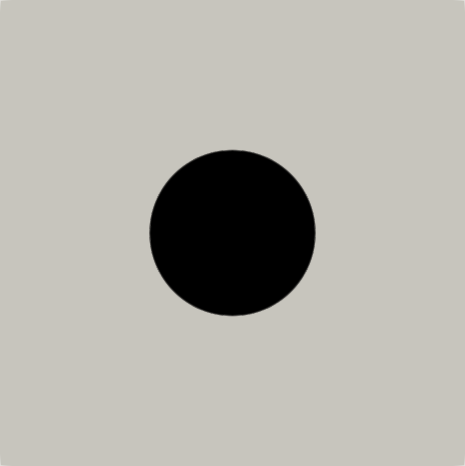
\includegraphics[width=0.35\textwidth]{fixfigs/ball-set.png} \qquad 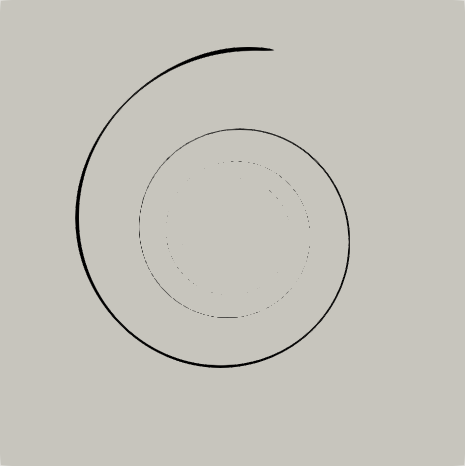
\includegraphics[width=0.35\textwidth]{fixfigs/spiral-set.png}
\end{center}
\caption{Coincidence sets for the ball and spiral problems in Example \ref{ex:results:classical}.}
\label{fig:results:classical}
\end{figure}

% see git@bitbucket.org:pefarrell/fascd.git: examples/drape.py
% and https://github.com/bueler/mcd-extended: paper/results/drape.sh|txt
\begin{table}[ht]
\begin{tabular}{lr@{\hskip 7mm}cccccc}
\toprule
\multirow{2}{*}{\emph{levels}} & \multirow{2}{*}{$m_J$} & \multicolumn{3}{c}{\,\emph{ball}} & \multicolumn{3}{c}{\,\emph{spiral}} \\ \cmidrule(lr){3-5} \cmidrule(lr){6-8}
   &          & V-cycle & F-cycle & RS only & V-cycle & F-cycle & RS only \\
\midrule
 1 &    $5^2$ &  1 &  1 &  1  &  1 &  1 &  1 \\
 2 &    $9^2$ &  2 &  1 &  2  &  2 &  1 &  2 \\
 3 &   $17^2$ &  2 &  2 &  3  &  3 &  2 &  4 \\
 4 &   $33^2$ &  3 &  2 &  6  &  3 &  2 &  7 \\
 5 &   $65^2$ &  3 &  2 &  8  &  4 &  3 &  9 \\
 6 &  $129^2$ &  4 &  2 & 17  &  4 &  3 & 16 \\
 7 &  $257^2$ &  4 &  2 & 33  &  4 &  3 & 27 \\
 8 &  $513^2$ &  5 &  2 & 65  &  5 &  3 & 48 \\
 9 & $1025^2$ &  5 &  2 & \XX &  5 &  3 & \XX \\
10 & $2049^2$ &  5 &  2 & \XX &  5 &  3 & \XX \\
\bottomrule
\end{tabular}
\bigskip
\caption{Iterations for FASCD V-cycle and F-cycle algorithms in Example \ref{ex:results:classical}.  Smoother-only runs marked \XX\xspace were not attempted.}
\label{tab:results:classical}
\end{table}

\begin{example}  \label{ex:results:plap}
We again consider Example \ref{ex:plaplacian} with a unilateral constraint, but now for the nonlinear $p$-Laplacian with both fast ($p=1.5$) and degenerate ($p=4.0$) diffusivities.\footnote{``Fast'' and ``degenerate'' refer to $|\grad u|^{p-2}\to \infty,0$, respectively; ellipticity is lost in the latter case.  Well-posedness and ($p$-dependent) solution regularity for $p$-Laplacian obstacle problems is considered in \cite{ChoeLewis1991}.} We consider the problem in one dimension for ease of visualization. This example reveals the sometimes strong contrast between $V(1,0)$ and $V(0,1)$ results (\pr{up}, \pr{down} $=0$ in Algorithm \ref{alg:fascd}, respectively), and it emphasizes the need for robust smoothers.

Set $\Omega=(-3,3)$, $\psi(x) = -0.2|x|$, $\mathcal{K} = \{v \ge \psi\} \subset W^{1,p}(\Omega)$, and $\ip\ell v = \int_\Omega g v$, where $g(x)=1$ for $|x|<1$ and $g(x)=-1$ for $|x|>1$, in VI \eqref{eq:vi}.  The exact solution is easily computed for any $p$; see Figure \ref{fig:results:plap} and the documentation of the code associated to this paper.  For this experiment we used a coarsest mesh of $m_0=7$ vertices and a finest mesh with $m_9=3073$.  The default smoother uses three (fixed) iterations of RS Newton, with LU solution of the arising linear systems, an $O(m_j)$ smoother in 1D.  The coarse solver is the same but iterated to convergence.  The initial iterate was $w=\psi$, and \texttt{rtol} $= 10^{-6}$ and \texttt{atol} $= 10^{-12}$.  Figure \ref{fig:imagesvcycle} illustrates the major steps of an example V-cycle, showing each of the coarse-correction VI subproblems and solutions.

%REGENERATE using elbueler/plapfigs branch of git@bitbucket.org:pefarrell/fascd.git, in examples/
% $ python3 plap1d.py -p 1.5 -figures -levs 6 -fascd_cycle_type full && mv solution.pdf plap1d1p5.pdf
% $ python3 plap1d.py -p 4.0 -figures -levs 6 -fascd_cycle_type full && mv solution.pdf plap1d4p0.pdf
\begin{figure}[ht]
\begin{center}
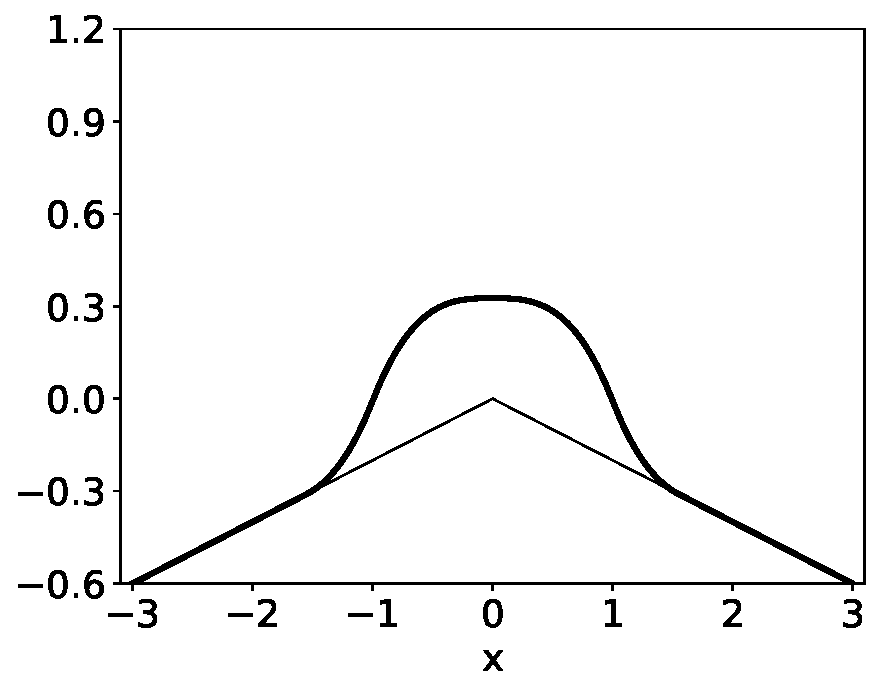
\includegraphics[width=0.45\textwidth]{fixfigs/plap1d1p5.pdf} \quad
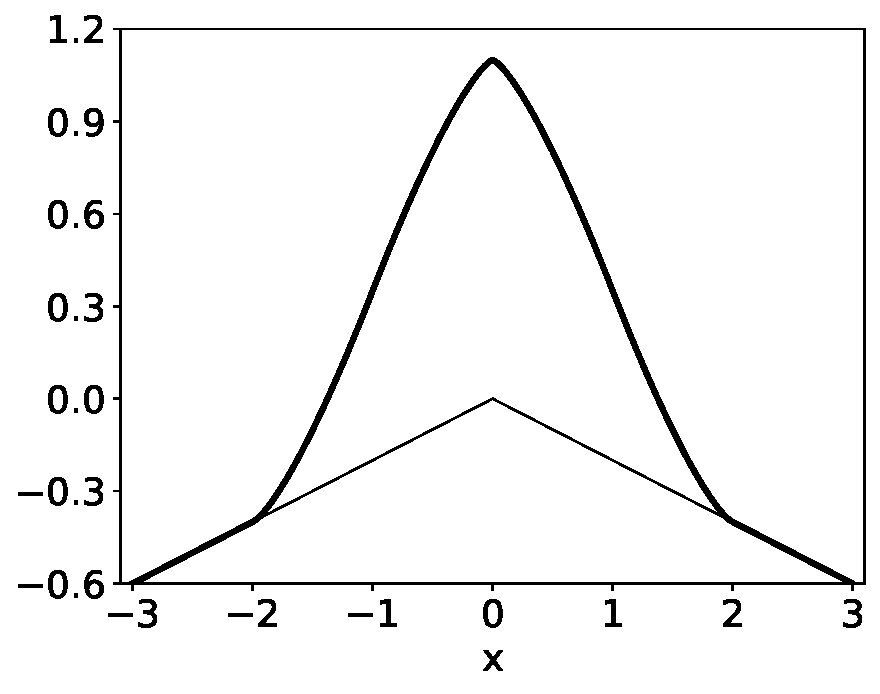
\includegraphics[width=0.45\textwidth]{fixfigs/plap1d4p0.pdf}
\end{center}
\caption{Solutions $u\ge \psi$ of the $p$-Laplacian VI in Example \ref{ex:results:plap}, for $p=1.5$ (left) and $p=4.0$ (right).}
\label{fig:results:plap}
\end{figure}

% figures in the following visualization were generated using branch elbueler/simplefigs
% of git@bitbucket.org:pefarrell/fascd.git, and the following commands (including imagemagick):
%   cd examples/
%   python3 plap1d.py -fascd_cycle_type multiplicative -mcoarse 4 -levs 3 -figures
%   [save the images into mcd-extended/paper/fixfigs/vcycle/]
%   for X in start2 down2 down1 up0 up1 up2 next2; do mogrify -trim $X.png $X.png; done
\begin{figure}[ht]
\begin{center}
\begin{tikzpicture}[scale=1.0]
    \pgfmathsetmacro{\HEIGHT}{2}
    \pgfmathsetmacro{\XSTEP}{3.7}
    \pgfmathsetmacro{\YSTEP}{3.7}
    \pgfmathsetmacro{\YLABEL}{-0.4}
    \pgfmathsetmacro{\NUDGE}{0.5}
    \node (start2) [] at (0,2*\YSTEP) {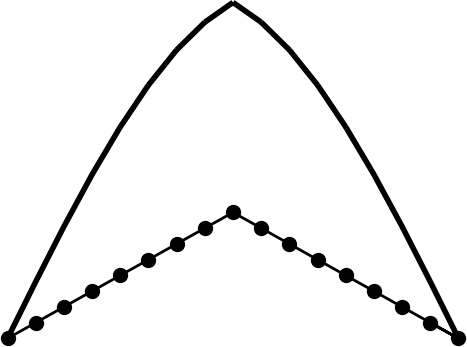
\includegraphics[height=\HEIGHT cm]{fixfigs/vcycle/start2.png}};
    \node (start2label) [below of = start2, yshift=\YLABEL cm] {$w^2 \ge \underline{\gamma}^2$};
    \node (down2) [] at (1.0*\XSTEP,2*\YSTEP) {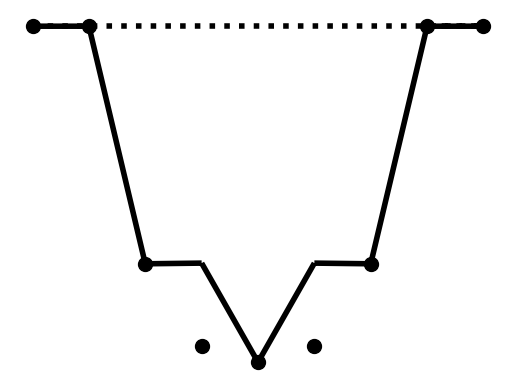
\includegraphics[height=\HEIGHT cm]{fixfigs/vcycle/down2.png}};
    \node (down2label) [below of = down2, yshift=\YLABEL cm] {$y^2 \ge \underline{\phi}^2$};
    \node (down1) [] at (1.4*\XSTEP,1*\YSTEP) {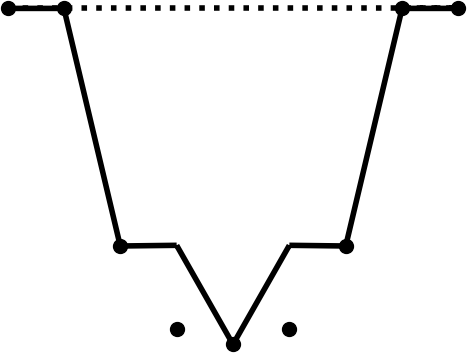
\includegraphics[height=\HEIGHT cm]{fixfigs/vcycle/down1.png}};
    \node (down1label) [below of = down1, yshift=\YLABEL cm] {$y^1 \ge \underline{\phi}^1$};
    \node (up0) [] at (1.9*\XSTEP,0) {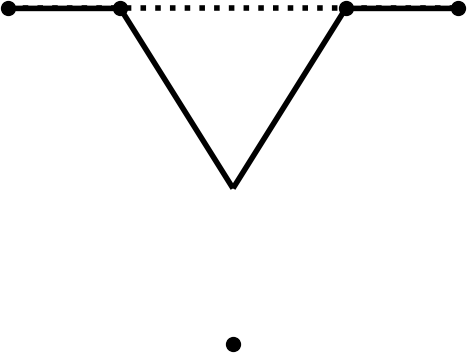
\includegraphics[height=\HEIGHT cm]{fixfigs/vcycle/up0.png}};
    \node (up0label) [below of = up0, yshift=\YLABEL cm] {$z^0 \ge \underline{\chi}^0$};
    \node (up1) [] at (2.4*\XSTEP,1*\YSTEP) {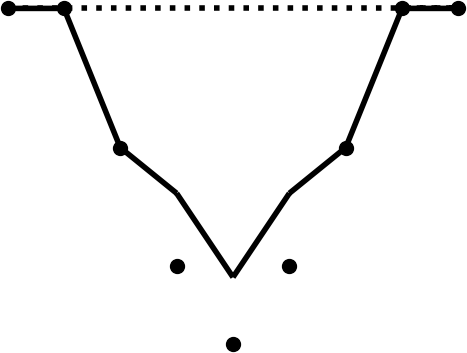
\includegraphics[height=\HEIGHT cm]{fixfigs/vcycle/up1.png}};
    \node (up1label) [below of = up1, yshift=\YLABEL cm] {$z^1 \ge \underline{\chi}^1$};
    \node (up2) [] at (2.8*\XSTEP,2*\YSTEP) {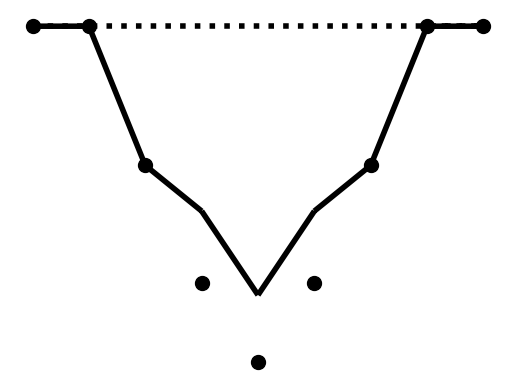
\includegraphics[height=\HEIGHT cm]{fixfigs/vcycle/up2.png}};
    \node (up2label) [below of = up2, yshift=\YLABEL cm] {$z^2 \ge \underline{\chi}^2$};
    \node (next2) [] at (3.8*\XSTEP,2*\YSTEP) {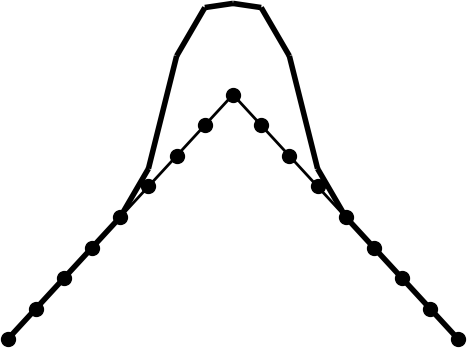
\includegraphics[height=\HEIGHT cm]{fixfigs/vcycle/next2.png}};
    \node (next2label) [below of = next2, yshift=\YLABEL cm] {$\tilde{w}^2 \ge \underline{\gamma}^2$};
    \graph [edges = {very thick}] {
        (start2) -> (down2)
                 -!- [] (down2label) -> (down1)
                 -!- [] (down1label) -> (up0)
                 -> (up1label) -!- (up1)
                 -> (up2label) -!- (up2)
                 -> (next2)
    };
\end{tikzpicture}

\end{center}
\caption{Visualization of one FASCD V-cycle iteration for Example \ref{ex:results:plap}, with $p=1.5$, $J=3$, and a coarsest mesh of $m_0=5$ vertices.  Solutions (i.e.~$w^j$, $y^j$, $z^j$) are lines, obstacles ($\underline{\gamma}^j$, $\underline{\phi}^j$, $\underline{\chi}^j$) are strong dots, and the zero function is dotted.  Vertical scale varies.}
\label{fig:imagesvcycle}
\end{figure}

Iteration results are shown in Table \ref{tab:results:fastplap1d} for the fast diffusion $p=1.5$ case.  We see that $V(1,0)$ cycles, essentially Algorithm 4.7 in \cite{GraeserKornhuber2009} but with a stronger smoother, often do not converge.  By contrast, $V(0,1)$ cycles, using only up-smoothing in the larger sets $\mathcal{U}^j$ (Section \ref{sec:cdmultilevel}), are just as good as the default $V(1,1)$ cycles ($=$ Algorithm \ref{alg:fascd}).  F-cycles are even more efficient except when they fail entirely, but these failures arise from singular diffusivity.  If we regularize  $D=|\grad u|^{-0.5}$ to $D_\eps = \left(\eps + |\grad u|^2\right)^{-0.25}$, with $\eps=10^{-8}$, then a single F-cycle suffices at every resolution (column ``F$_\eps$'').

Iteration results for the (unregularized) degenerate diffusion $p=4.0$ case are in Table \ref{tab:results:degenerateplap1d}.  V-cycles using the default settings, specifically three fixed RS Newton iterations, do not converge on the finer meshes; the semi-smooth NCP residual norms \eqref{eq:stoppingcriterion} are unbounded in the failed runs.  Visualization shows an instability in which oscillations in the restricted residuals explode.  However, either a slight increase in smoother power, to four RS Newton iterations, or improved finest-level initial iterates through use of an F-cycle, stops the instability.  Even for the three-iteration smoother, a single F-cycle suffices at every resolution.

The $p=1.5$ and $p=4$ cases give different convergence rates in the $\|\cdot\|_\infty$ norm, namely at rates $O(h^{2.005})$ and $O(h^{1.420})$, respectively; compare \cite{ChoeLewis1991}.
\end{example}

% see git@bitbucket.org:pefarrell/fascd.git: examples/plap1d.py
% and https://github.com/bueler/mcd-extended: paper/results/plap1d.sh|txt
\begin{table}[ht]
\begin{tabular}{lr@{\hskip 7mm}c@{\hskip 3mm}c@{\hskip 3mm}c@{\hskip 4mm}c@{\hskip 5mm}c@{\hskip 6mm}c}
\toprule
\emph{levels} & $m_J$ & V(1,0) & V(0,1) & V(1,1) & F & F$_\eps$ & $\|$error$\|_\infty$ \\
\midrule
 1 &    $7$ &  1 &  1 &  1 &  1 &  1 & $2.3\times 10^{-1}$ \\
 2 &   $13$ &  3 &  3 &  2 &  2 &  1 & $3.3 \times 10^{-2}$ \\
 3 &   $25$ & 12 &  4 &  2 &  1 &  1 & $9.1 \times 10^{-3}$ \\
 4 &   $49$ & NC &  4 &  2 &  1 &  1 & $3.2 \times 10^{-3}$ \\
 5 &   $97$ & NC &  3 &  3 &  1 &  1 & $5.5 \times 10^{-4}$ \\
 6 &  $193$ & NC &  3 &  3 & NC &  1 & $1.7 \times 10^{-4}$ \\
 7 &  $385$ & NC &  3 &  3 &  1 &  1 & $4.7 \times 10^{-5}$ \\
 8 &  $769$ & NC &  4 &  7 &  1 &  1 & $9.5 \times 10^{-6}$ \\
 9 & $1537$ & NC &  5 &  6 & NC &  1 & $3.6 \times 10^{-6}$ \\
10 & $3073$ & NC & 11 & 19 &  1 &  1 & $4.9 \times 10^{-7}$ \\
\bottomrule
\end{tabular}
\bigskip
\caption{Iterations for V- and F-cycles on the $p=1.5$ problem in Example \ref{ex:results:plap}.  NC $=$ did not converge after 50 iterations.  See text regarding F$_\eps$ and error.}
\label{tab:results:fastplap1d}
\end{table}

% see git@bitbucket.org:pefarrell/fascd.git: examples/plap1d.py
% and https://github.com/bueler/mcd-extended: paper/results/plap1d.sh|txt
\begin{table}[ht]
\begin{tabular}{lr@{\hskip 7mm}c@{\hskip 4mm}c@{\hskip 4mm}c@{\hskip 6mm}c}
\toprule
\emph{levels} & $m_J$ & V & V$_4$ & F & $\|$error$\|_\infty$ \\
\midrule
 1 &    $7$ &  1 &  1 &  1 & $8.7 \times 10^{-2}$ \\
 2 &   $13$ &  1 &  1 &  1 & $3.8 \times 10^{-2}$ \\
 3 &   $25$ &  2 &  1 &  1 & $1.6 \times 10^{-2}$ \\
 4 &   $49$ &  4 &  2 &  1 & $6.3 \times 10^{-3}$ \\
 5 &   $97$ & NC &  2 &  1 & $2.3 \times 10^{-3}$ \\
 6 &  $193$ & NC &  1 &  1 & $7.0 \times 10^{-4}$ \\
 7 &  $385$ & NC &  2 &  1 & $2.0 \times 10^{-4}$ \\
 8 &  $769$ & NC &  2 &  1 & $1.1 \times 10^{-4}$ \\
 9 & $1537$ & NC &  2 &  1 & $4.0 \times 10^{-5}$ \\
10 & $3073$ & NC &  2 &  1 & $1.5 \times 10^{-5}$ \\
\bottomrule
\end{tabular}
\bigskip
\caption{Iterations for V- and F-cycles on the $p=4.0$ problem in Example \ref{ex:results:plap}.  See text regarding V$_4$ and error.}
\label{tab:results:degenerateplap1d}
\end{table}

Solvers implemented in Firedrake can exploit parallel solvers from the PETSc library \cite{Balayetal2023}, and in fact the above Examples, which were run in serial so as to fix the smoother, also run efficiently in parallel.  The next Examples apply parallel solvers, and Example \ref{ex:results:sia} demonstrates the parallel weak scaling \cite{Bueler2021} of FASCD.

\begin{example}  \label{ex:results:advdiff}
Consider the advection-diffusion VI problem in Example \ref{ex:advectiondiffusion} with $\Omega=(-1,1)^d$, $d=2,3$, diffusivity $\eps=0.1$ in equation \eqref{eq:advectiondiffusionstrong}, and zero Dirichlet boundary conditions.  We made the 2D problem satisfy the coercivity hypothesis with a divergence-free velocity field $\bX = (7+5y,-5x)$, but in 3D, for variety's sake, we set $\bX = (7+5y,-5x,2z)$ so $\grad\cdot\bX \ne 0$.  The chosen discontinuous source term $\phi \in L^\infty(\Omega)$ satisfies $\phi\ge 0$ in half of the domain, with positive circular patches, with negative values in the other half; details are in the associated code.  While the other Examples in this Section are unilateral, here the solution is box-constrained: $0 \le u \le 1$.  Figure \ref{fig:results:advdiff} shows coincidence sets for the 2D problem; the 3D sets are comparable in regularity and general pattern.

% REGENERATE using git@bitbucket.org:pefarrell/fascd.git, in examples/
%   mpiexec -n 16 --map-by core --bind-to hwthread python3 pollutant.py -dim 2 -levs 7 -o poll2d.pvd
%   paraview poll2d.pvd
% to plot coincidence sets use ranges 0 <= u <= 0.00001 and 0.99999 <= u <= 1 and
% preset "xray" and invert colors (for u=0) or keep colors (u=1)
\begin{figure}[ht]
\begin{center}

\includegraphics[width=0.35\textwidth]{fixfigs/poll2d-zero-set.png} \qquad 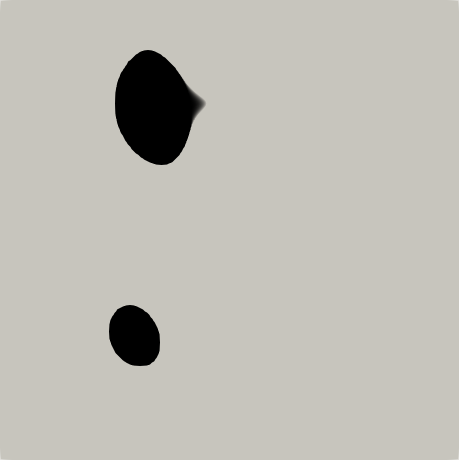
\includegraphics[width=0.35\textwidth]{fixfigs/poll2d-one-set.png}
\end{center}
\caption{Coincidence sets for the 2D bi-obstacle problem in Example \ref{ex:results:advdiff}: $u=0$ (left) and $u=1$ (right).}
\label{fig:results:advdiff}
\end{figure}

The 2D solver applied $P_1$ elements and a single processor, but in 3D the elements were chosen to be $Q_1$ (hexahedra) and the run parallel ($P=16$ processes).  A coarse mesh with $m_0=16^d$ vertices minimally-resolved the coincidence set.  The smoother was two (fixed) RS Newton iterations, with three preconditioned GMRES iterations to approximately solve the arising linear systems; the preconditioning was additive Schwarz method (ASM) with incomplete factorization (ILU) on each process.  The coarse solver was RS Newton and LU, iterated to convergence.  Tolerances \id{rtol} $=10^{-5}$ and \id{atol} $=10^{-9}$ were used in \eqref{eq:stoppingcriterion}.

F-cycle iteration results are shown in Table \ref{tab:results:advdiff}.  Despite the hint of growing iterations under mesh refinement, a few iterations sufficed up to memory-limited resolutions.  For any of the higher resolution runs, the FASCD F-cycle solver took less time than generating the mesh hierarchy.  The local Péclet number $\text{Pe}=\|\bX(x,y,z)\|_2 L \eps^{-1}$, with $L=2$ the width of $\Omega$, varied from 40 to 260.  The mesh Péclet number $m_J^{-1/d}\,\text{Pe}$ varied accordingly, and though the $m_J\le 121^d$ problems were advection-dominated, those with $m_J\ge 481^d$ were diffusion-dominated, and the smoother was the same in all cases, with nearly-constant iterations.
\end{example}

% see git@bitbucket.org:pefarrell/fascd.git: examples/pollutant.py
% and https://github.com/bueler/mcd-extended: paper/results/pollutant.sh|txt
\begin{table}[ht]
\begin{tabular}{lr@{\hskip 7mm}c@{\hskip 4mm}c}
\toprule
\emph{levels} & $m_J$ & $d=2$ & $d=3$ \\
\midrule
 1 &    $16^d$ & 1 & 1 \\
 2 &    $31^d$ & 2 & 2 \\
 3 &    $61^d$ & 2 & 2 \\
 4 &   $121^d$ & 2 & 2 \\
 5 &   $241^d$ & 2 & 3 \\
 6 &   $481^d$ & 2 \\
 7 &   $961^d$ & 3 \\
 8 &  $1921^d$ & 3 \\
 9 &  $3841^d$ & 3 \\
\bottomrule
\end{tabular}
\bigskip
\caption{F-cycle iterations for 2D ($P_1$, serial) and 3D ($Q_1$, 16 processes) solutions of the advection-diffusion bi-obstacle VI problem in Example \ref{ex:results:advdiff}.}
\label{tab:results:advdiff}
\end{table}

\begin{example}   \label{ex:results:sia}
We consider the steady shallow ice approximation (SIA) obstacle problem presented in Example \ref{ex:sia}, in which the surface elevation is constrained to exceed the bedrock elevation, $s\ge b$.  We set $\Omega=(0,L)^2$ with $L=1800$ km.  The data consist of a radial surface mass balance function $a$ \cite[equation (5.122)]{GreveBlatter2009} and a bumpy, synthetic map $b\in C^1(\Omega)$, with an elevation range of $1800$ m; details for $b$ are in the associated code.  A numerical solution is shown in Figure \ref{fig:results:siascene}, colored by the solution surface flow speed, i.e.~the magnitude of $\mathbf{u} = (n+1)(n+2)^{-1} \Gamma (s-b)^{n+1} |\grad s|^{n-1} \grad s$.  As noted in Example \ref{ex:sia}, and seen in this Figure, $|\grad s|$ is unbounded at the free boundary; the solution $s$, while continuous, has very low regularity.

% to regenerate from git@bitbucket.org:pefarrell/fascd.git: examples/:
%   $ mpiexec -n 16 --map-by core --bind-to hwthread python3 sia.py -levs 8 -bumps \
%       -mcoarse 8 -fascd_cycle_type full -fascd_monitor -fascd_rtol 2.0e-4 \
%       -fascd_atol 1.0e-8 -o sialev8.pvd
\begin{figure}[ht]
\begin{center}
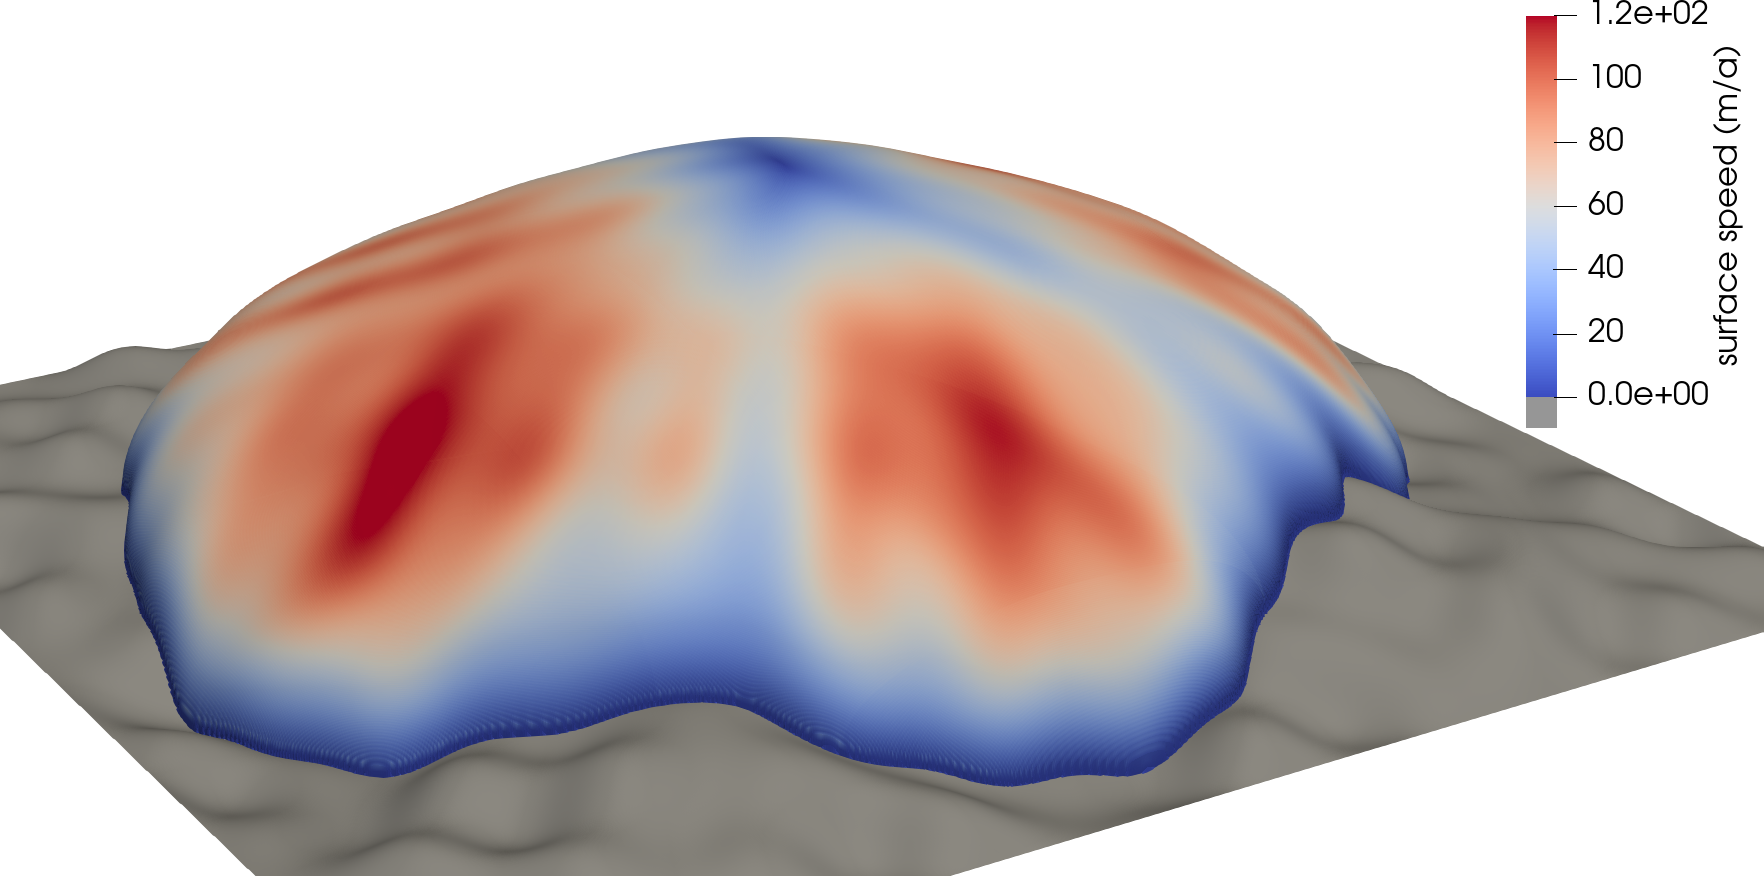
\includegraphics[width=1.0\textwidth]{fixfigs/sialev8scene.png}
\end{center}
\caption{Solution of Example \ref{ex:sia} over a bumpy bedrock topography (grey), with the ice speed as surface coloring and 100-times vertical exaggeration.}
\label{fig:results:siascene}
\end{figure}

We applied FASCD F-cycles using $Q_1$ elements and a smoother of four (fixed) iterations of RS Newton (Section \ref{sec:implementation}), with quadratic backtracking line search.  The arising linear systems were approximately solved, in parallel, by three (fixed) iterations of preconditioned GMRES and a ASM+ILU preconditioner.  The coarse solver was RS+LU, applied redundantly over all processors.  The coarse mesh was relatively fine, with $m_0=21^2$ vertices and 400 cells.  Because of the low regularity of the solution we used \id{rtol} $= 2 \times 10^{-4}$ and \id{atol} $= 10^{-8}$ in \eqref{eq:stoppingcriterion}.  The initial iterate was zero ice: $s=b$.  These parameters generated a solver with mesh-independent iterations.

For a weak-scaling study we fixed the number of degrees of freedom per process at $m_J/P=641^2 \approx 4.1 \times 10^5$ and solved with $6, \dots, 11$ refinements.\footnote{The experiments were conducted on ARCHER2, the UK national supercomputer. Each node has 16 memory channels, so a maximum of 16 cores per node were employed.}  The results in Table \ref{tab:results:siaweak} show some degradation in time per cycle with increasing core counts, perhaps due to the use of one-level additive Schwarz in the solution of the arising linear systems. Nevertheless, the finest mesh result, with $m_J=20481^2=4.1 \times 10^8$ degrees of freedom, required less than three minutes to solve for the steady surface elevation of an ice sheet larger than the current Greenland ice sheet ($1.7$ million $\text{km}^2$) at uniform $87.5$ m resolution.
\end{example}

% see git@bitbucket.org:pefarrell/fascd.git: examples/sia.py
% and https://github.com/bueler/mcd-extended: paper/results/siaweak.sh|txt
\begin{table}[ht]
\begin{tabular}{c@{\hskip 4mm}c@{\hskip 4mm}c@{\hskip 7mm}c@{\hskip 4mm}c}
\toprule
$P$ & \emph{levels} & $m_J$ & \emph{F-cycles} & \emph{time} (s) \\
\midrule
 1 & 6 & $641^2$ & 3 & 98 \\
 4 & 7 & $1281^2$ & 3 & 98 \\
 16 & 8 & $2561^2$ & 3 & 124 \\
 64 & 9 & $5121^2$ & 3 & 136 \\
 256 & 10 & $10241^2$ & 2 & 95 \\
 1024 & 11 & $20481^2$ & 2 & 177 \\
 \bottomrule
\end{tabular}
\bigskip
\caption{Iterations and run time (wall clock, in seconds) for parallel FASCD F-cycle solutions of Example \ref{ex:sia} on $P$ processes.}
\label{tab:results:siaweak}
\end{table}

\elb{beam example?}


\section{Discussion and outlook} \label{sec:discussion}

As a multilevel solver for VI problems, one might describe the new FASCD method as merely a strategy for generating coarser-level problems which, once solved, make helpful admissible additions to a final V-cycle update.  The method is smoother-agnostic, and our implementation within the extensible Firedrake \cite{Rathgeberetal2016} and PETSc \cite{Balayetal2023} library framework should allow easy experimentation with other smoothers (projected Gauss--Seidel, semi-smooth Newton, interior-point, etc.), beyond the active-set Newton method \cite{BensonMunson2006} chosen for demonstration here.  For box-constrained smoothers of Newton-Krylov type one could also add linear geometric or algebraic multigrid preconditioning \cite{Trottenbergetal2001}, instead of our simple choice of incomplete factorization and (in parallel) additive Schwarz preconditioners.  Thus there is a large smoother and coarse solver space to explore.  However, the performance of the particular method shown in Section \ref{sec:results} is already excellent.

The observation that up-smoothing is more efficient in a multilevel CD context, which arises because of constraint set distinctions, seems to be new, but compare comments on $V(1,1)$ cycles in \cite{GraeserKornhuber2009,Tai2003}.  The increased efficiency is particularly shown in Example \ref{ex:results:plap}.  In summary, the distinction is that construction of constraint sets via monotone injection generates up-smoothing sets which can telescope the down-smoothing sets (Lemma \ref{lem:upwardadmissibility}); we call this an \emph{incomplete CD}.  This structure can be exploited by a new CD iteration, algorithm \pr{icd-tele} in Section \ref{sec:cdmultilevel}.

In contrast with monotone multigrid \cite{Kornhuber1994}, FASCD does not modify the FE discretization, but the possibility of acceleration via basis-level manipulations is a topic for future research.  On the other hand,  the convergence proofs in \cite{GraeserKornhuber2009,Kornhuber1994}, which appear to depend on particular smoother and basis-level manipulation choices, have no analog here.


\subsection*{Code availability} \label{sec:code}  The software used to produce the results is archived at tag \elb{FIX} in the repository \url{https://bitbucket.org/pefarrell/fascd/}, using the Firedrake version \elb{what version?}


\subsection*{Acknowledgements} \label{sec:acknowledgements}  EB was supported by a Faculty Development Travel Award from United Academics, University of Alaska Fairbanks. PEF was supported by the Engineering and Physical Sciences Research Council [EPSRC grants EP/R029423/1 and EP/W026163/1]. This work used the ARCHER2 UK National Supercomputing Service (https://www.archer2.ac.uk). PEF thanks Jack D.~Betteridge for assistance with the numerical experiments of Section \ref{ex:results:sia}.



\bibliography{fascd}
\bibliographystyle{siam}


\appendix
\section{Reduction to FAS multigrid for PDEs} \label{app:reductions}

When all inequality constraints are removed the FASCD V-cycle Algorithm \ref{alg:fascd} reduces to the classical FAS multigrid V-cycle for nonlinear PDEs \cite{Brandt1977,Trottenbergetal2001}, which itself generalizes linear multigrid.  In fact, suppose we replace $\underline{\gamma}^J,\overline{\gamma}^J$ in definition \eqref{eq:fe:fineconstraintset} with $-\infty,+\infty$, respectively.  The finest-level admissible set $\mathcal{K}^J$ is then determined only by the Dirichlet boundary conditions.  Let $\mathcal{V}_0^J \subset \mathcal{V}^J$ denote the linear subspace with zero values on $\partial_D\Omega$.  Since $v-u^J\in\mathcal{V}_0^J$ is now arbitrary we can rewrite \eqref{eq:fe:vi} as the FE discretization of strong-form PDE $f(u)=\ell$: find $u^J \in \mathcal{V}^J$ such that
\begin{equation}
\ip{f^J(u^J)}{v} = \ip{\ell^J}{v} \qquad \text{for all } v\in \mathcal{V}_0^J. \label{eq:app:fas:pde}
\end{equation}

The downward $\mathcal{D}^j$ and upward $\mathcal{U}^j$ constraint sets are also enlarged to vector spaces, and the corrections $y^j$ and $z^j$ are unconstrained; lines \ref{line:vcyclegenchifinest}, \ref{line:vcyclegenchi}, and \ref{line:vcyclegenphi} in Algorithm \ref{alg:fascd} can be removed.  Then VI problems \eqref{eq:fe:downvi} and \eqref{eq:fe:upvi} can be rewritten as the weak form problem $\ip{f^j(u^j)}{v} = \ip{\ell^j}{v}$ over $v\in \mathcal{V}_0^j$, where $u^j=w^j+y^j$ when down-smoothing and $u^j=w^j+z^j$ when up-smoothing, and the smoothers can be regarded as unconstrained, in-place modifications of $u^j$.  Noting line \ref{line:vcyclerestrictsolution} now says $u^{j-1}=\iR u^j$, after down-smoothing the coarsened source functional computed by line \ref{line:vcyclerestrictell} can be rewritten as $\ell^{j-1} = f^{j-1}\left(u^{j-1}\right) + R\left(\ell^j-f^j(u^j)\right)$.

Going upward we must be careful that only the coarse correction, and not the coarse solution, is prolonged \cite[remark 5.3.9]{Trottenbergetal2001}.  After up-smoothing on the $j-1$ level the coarse iterate is $u^{j-1}$, but at this point $u^j=w^j + y^j$ contains the result of $j$th-level down-smoothing.  The initial value of the correction $z^j$, before up-smoothing on the $j$th level, is $z^j = y^j + P z^{j-1}$, where $z^{j-1}$ contains the total correction from coarser corrections and $j-1$ level up-smoothing.  Thus the $j$th-level iterate \emph{before} up-smoothing must be set to $w^j + y^j + P z^{j-1} = u^j + P(u^{j-1} - \iR u^j)$, which replaces line \ref{line:vcycleupsmoothinitial}.

With these modifications, Algorithm \ref{alg:fascd} becomes the FAS V-cycle below, as a solver for \eqref{eq:app:fas:pde}.  It appears in various literature, for example \cite[Algorithm 14]{Bruneetal2015} and \cite[section 5.3.4]{Trottenbergetal2001}.

\begin{pseudo*}
\pr{fas-vcycle}(\ell^J; u^J)\text{:} \\+
    for $j=J$ downto $j=1$ \\+
      $\text{\pr{smooth}}^{\text{\id{down}}}(\ell^j;u^j)$ \\
      $u^{j-1} = \iR u^j$ \\
      $\ell^{j-1} = f^{j-1}(u^{j-1}) + R \left(\ell^j - f^j(u^j)\right)$ \\-
    $\text{\pr{solve}}(\ell^0;u^0)$ \\
    for $j=1$ to $j=J$ \\+
      $u^j \gets u^j + P (u^{j-1} - \iR u^j)$ \\
      $\text{\pr{smooth}}^{\text{\id{up}}}(\ell^j;u^j)$ \\-
\end{pseudo*}

\end{document}
